\chapter[Extraction of Generalized Polarization Tensors]
{Extraction of Generalized Polarization Tensors
\chapsubhead{The results of this chapter have been submitted in \cite{ABGJKW2012dico} and \cite{ammari2012tracking}.}}

\label{chap:GPT-extraction}

\begin{abstract}
In order to recognize the shape of a target, we will need to develop tools
that are not available in the literature. This will not only help
us for the electrolocation problem, but it will also advance the more general
field of mathematical imaging and numerical inverse problems. Hence, in
chapters~\ref{chap:GPT-extraction}-\ref{chap:tracking}, we will take away from
the electrolocation problem to go to a canonical setting in electro-sensing.

In this chapter, we will develop tools to extract, from multi-static measurements,
physically relevant features called Generalized Polarization Tensors (GPTs).
The system has the remarkable property that low order generalized
polarization tensors are not affected by the error caused by  the
instability of higher orders in the presence of measurement noise.
This will later enables us to identify an object thanks to a dictionary
(chapter~\ref{chap:dico-matching}) and tracking it when moving (chapter~\ref{chap:tracking}).
We will study the full-view and partial-aperture problems, since they will be important
for later application on active electrolocation (chapter~\ref{chap:pnas}).
\end{abstract}

%%%%%%%%%%%%%%
\section{Introduction}\label{sec:introduction}

With each domain and material parameter, an infinite number of
tensors, called the Generalized Polarization Tensors (GPTs), is
associated. The concept of GPTs was introduced in
\cite{ammarisima02, ammari2004reconstruction}. The GPTs contain significant information
on the shape of the domain \cite{AK_MMS_03}. It occurs in several
interesting contexts, in particular, in low-frequency scattering
\cite{dassios, ammari2004reconstruction}, asymptotic models of dilute composites (see
\cite{milton2002theory} and \cite{AKT_AA_05}), in invisibility cloaking in
the quasi-static regime \cite{AKLL11} and in potential theory
related to certain questions arising in hydrodynamics \cite{PS51}.

 In fact, the GPTs are
the basic building blocks for the asymptotic expansions of the
boundary voltage perturbations due to the presence of small
conductivity inclusions inside a conductor \cite{FV_ARMA_89,cedio1998identification,
ammarisima02}. In other words, the dipole approximation computed in
section~\ref{sec:perturbation-target} is the first order approximation of a more
general expansion involving these GPTs that will be expressed here.

The GPTs can be
accurately obtained from multistatic measurements by solving a
linear system. We provide here a stability analysis for the reconstruction of
the GPTs in the presence of measurement noise and with respect to the aperture
angle formed by the sources/receptors array. This will quantify the
ill-posedness of the imaging problem.


The chapter is organized as follows. In section
\ref{sec:struct-mult-resp}, we introduce a particular linear
combination of the GPTs  to obtain what we call the contracted
GPTs (CGPTs) \cite{AKLL11}. In Section
\ref{sec:reconstr-cgpt-stab}, we investigate the reconstruction of
contracted GPTs, defined in \eqref{defc1}--\eqref{defc2} below,
from the multistatic response matrix of a conductivity problem. We
also consider the effect of the presence of measurement noise in
the MSR (subsection~\ref{sub:electronic-noise}) and aperture 
(subsection~\ref{sec:limited_angle_view}) on the reconstruction of the CGPTs. Given a
signal-to-noise ratio, we determine  the statistical stability in
the reconstruction of the CGPTs, and show that such inverse
problem is exponentially unstable. This is the well-known
ill-posedness of the inverse conductivity problem. Numerical results are
summarized in section~\ref{sec:results-GPT-extraction}.

\section{Structure of the Multistatic Response Matrix}\label{sec:struct-mult-resp}

Here we propose to reconstruct CGPTs from the
multistatic response  (MSR) matrix, which measures the change in
potential field due to a conductivity inclusion. In this section,
we present the toy model for MSR and write it in terms of
the CGPTs associated to the conductivity inclusion.

In order to take into account the similarity between the EIT setting and the
electrolocation problem, the notations will be quite the same as in chapter~\ref{chap:math-model}. 
We consider a two dimensional conductivity medium with uniform
conductivity equal to one, except in an inclusion where the
conductivity is $k
> 1$; we denote by $\lambda$ the contrast of this inclusion, that
is,  $\lambda = (k + 1)/(2(k - 1))$. To this point, let us remark that for
application to the electrolocation problem, we will need $k \in \mathbb{C}$. This
problem will be tackled in chapter~\ref{chap:pnas}, but for the moment we will restrict
ourselves to the real case, since in this case we have much more properties
(such as symmetry for example~\cite{ammari2007polarization}).
Let $D = z + \delta
B = \{ x = z + \delta y ~|~ y \in B\}$ model the conductivity
inclusion.  Here, $B$ is some $\mathcal{C}^2$ and bounded domain
in $\R^2$ whose typical length scale is of order one; $z$ is a
point in $\R^2$ and is taken here to be an estimation of the
location of the inclusion; $\delta$ is the typical length scale of
the inclusion. We refer to \cite{ammari2004reconstruction} for efficient location
search algorithms and to \cite{AGJ} for correcting the effect of
measurement noise on the localization procedure.

The MSR matrix is constructed as follows. Let
$\{x_r\}_{r=1}^{N_r}$ and $\{x_s\}_{s=1}^{N_s}$ model a set of
electric potential point detectors and electric point sources. We
assume in this chapter that the two sets of locations coincide and
$N_r = N_s = N$ (see an example in Figure~\ref{fig:example-configuration-MSR-EIT}).
The MSR matrix $\mathbf{V}$ is an $N$-by-$N$
matrix whose $rs$-element is the difference of electric potentials
with and without the conductivity inclusions:
\begin{equation}
V_{rs} = u_s(x_r) - G_s(x_r), \quad r, s = 1, \ldots, N.
\end{equation}
Here, $G_s (x) = G(x-x_s)$ and $G(x) =
\frac{1}{2\pi} \log |x|$ is the fundamental solution of the
Laplace equation in $\R^2$, and $u_s(x)$ is the solution to the
transmission problem
\begin{equation}
\left\{
\begin{aligned}
\nabla \cdot (1 + (k-1) \chi_{D}) \nabla u_s(x) &= \delta_{x_s}(x),  & & x \in \R^2 \backslash \partial D,\\
u_s (x) \big|_{+} &= u_s (x) \big|_{-}, & & x \in \partial D,\\
\nu_x \cdot (\nabla u_s) \big|_{+} &= k \nu_x \cdot (\nabla u_s) \big|_{-}, & & x \in \partial D,\\
u_s(x) - G_s (x) & = \mathcal{O}(|x|^{-1}), & & |x-x_s| \to
\infty.
\end{aligned}
\right. \label{eq:transm}
\end{equation}
In the second and third equations above, the notation
$\phi\big|_{\pm}(x)$ denotes the limit $\lim_{t \downarrow 0}
\phi(x\pm t\nu_x)$, where $x \in \partial D$ and $\nu_x$ is the
outward unit normal of $\partial D$ at $x$.

\begin{figure}[htp]
  \centering
  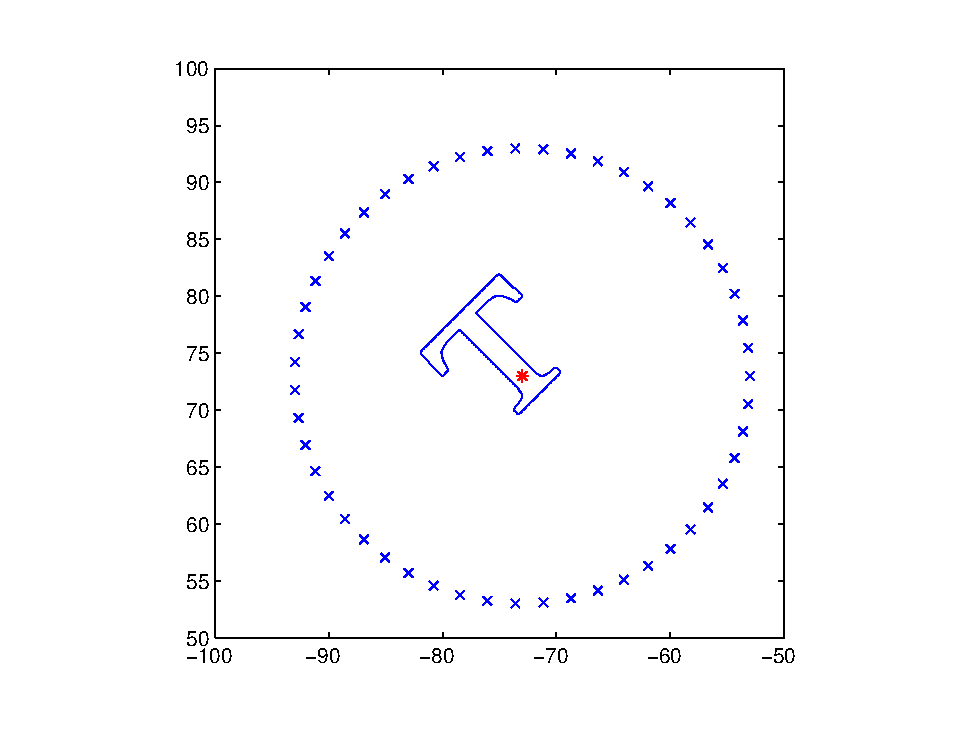
\includegraphics[width=\textwidth]{dico/figures/fig1}
  \caption{An example of configuration for MSR data simulation. Here,
  the unknown shape
  is a rotated letter ``T''. $N=51$
  sources/receivers marked by ``x'' are equally placed on a circle
  of radius $R=20$ centered at $z_0=[-73, 73]$ which is marked by
  ``*''.}
  \label{fig:example-configuration-MSR-EIT}
\end{figure}

Let us remark that the system~(\ref{eq:transm}) is closely related to
system~(\ref{eq:direct_problem-final}) of chapter~\ref{chap:math-model}. Indeed,
here $u_s$ is the electric potential coming from a point source at $x_s$ whereas
in system~(\ref{eq:direct_problem-final}), $u$ is the electric potential given by
the sum of Dirac masses (or the dipole) denoted $J_s$. Hence, the difference is
here that we have several sources~; as mentioned in section~\ref{sec:intro-localization},
this was the major difficulty in chapter~\ref{chap:localization}.


%%%%%%%%%
\subsection{The asymptotic expansion of the perturbed potential field}

\label{sub:asymptotic-expansion-perturbed-potential-field}

As modeled above, the MSR matrix characterizes the perturbed
potential field $u_s(x_r) - G_s(x_r)$. In this section we
recall, from \cite{ammari2004reconstruction},  the asymptotic expansion of this
perturbation and that generalize those in chapter~\ref{chap:math-model}.

First, let us explicit the layer potential operators (define 
section~\ref{sub:existence-uniqueness}) with these new notations.
Let $\mathcal{S}_D$ be the single layer potential associated with
$D$, that is,
\begin{equation}
\mathcal{S}_D[\phi](x) :  = \int_{\partial D} G(x-y) \phi(y)
ds(y), \quad x \in \R^2,
\end{equation}
and let $\mathcal{K}_D: L^2(\partial D) \to L^2(\partial D)$
denote the Poincar\'e-Neumann operator
\begin{equation}
\mathcal{K}_D[\phi] (x) : = \frac{1}{2 \pi} \int_{\partial D}
\frac{\langle y - x, \nu_y\rangle}{|x-y|^2} \phi(y) ds(y), \quad x
\in \partial D. \label{eq:Kdef}
\end{equation}
Here $\nu_y$ is the unit normal vector along the boundary at $y$. Relation
\ref{eq:jump_formulas} gives us $\mathcal{S}_D[\phi]\big|_- =
\mathcal{S}_D[\phi]\big|_+$ and the jump condition
\begin{equation}
\frac{\partial}{\partial \nu} \mathcal{S}_D[\phi] \Big|_{\pm} =
\left( \pm \frac{1}{2} I + \mathcal{K}_D^*  \right)[\phi],
\label{eq:Sjump}
\end{equation}
where $\mathcal{K}_D^*$ is the adjoint operator of $\mathcal{K}_D$~;
it has a similar expression as \eqref{eq:Kdef} with the
numerator of the integrand replaced by $\langle x - y,
\nu_x\rangle$. Using \eqref{eq:Sjump}, we verify that $G_s(x)
+ \mathcal{S}_D[\phi_s]$ with $\phi_s \in L^2(\partial D)$ solving
\begin{equation}
\left( \lambda I - \mathcal{K}_D^* \right)[\phi_s] =
\frac{\partial G_s}{\partial \nu} \Big|_{\partial D},
\end{equation}
is a solution to the transmission problem \eqref{eq:transm}. In
fact, this solution is unique and we conclude that
\begin{equation}
u_s(x) - G_s(x) = \mathcal{S}_D[\phi_s] = \int_{\partial D}
G(x - y) (\lambda I - \mathcal{K}_D^*)^{-1}
\bigg[\frac{\partial G_s}{\partial \nu}\Big|_{\partial D}
\bigg](y)  ds(y). \label{eq:dfield}
\end{equation}
To verify the formal derivation above, we refer the reader to
Section 2.4 of \cite{ammari2004reconstruction}.

Throughout this section, we use Greek letters to denote double
indices: $\alpha = (\alpha_1, \alpha_2) \in \mathbb{N}^2$,
$\alpha! = \alpha_1 ! \alpha_2 !$, $|\alpha| = \alpha_1 +
\alpha_2$, $x^\alpha = x_1^{\alpha_1} x_2^{\alpha_2}$,
and $\partial^\alpha = \partial_1^{\alpha_1}
\partial_2^{\alpha_2},$ with $\partial_j = \partial /
\partial x_j$.

We assume that the inclusion $D$ and the point $z$ is away from
the sources. As a result, the functions $G(x_r - y)$ and
$G_s(y)$ are smooth for $y \in \overline{D}$, and the
perturbed field \eqref{eq:dfield} is well defined. For $y \in
\partial D$ and $z$ away from $x$, the $K$-th order Taylor
expansion formula with remainder $e_K$ states
\begin{equation}
G(x - y) = G(x - z - (y-z)) = \sum_{|\alpha| = 0}^K
\frac{(-1)^{|\alpha|}}{\alpha!} \partial^{\alpha} G(x - z)
(y-z)^\alpha + e_K.
\end{equation}
Substitution of this expansion into \eqref{eq:dfield}
yields the following expansion of $V_{rs}$ plus an error term
denoted by $E_{rs}$:
\begin{equation*}
V_{rs}= \sum_{|\alpha|,|\beta|=1}^K \frac{(-1)^{|\alpha|}}{\alpha
! \beta !} \partial^\alpha G(x_r-z) Q_{\alpha\beta}(z)
\partial^\beta G(z-x_s) + E_{rs},
\end{equation*}
with
$$
Q_{\alpha\beta}(z)= \int_{\partial D} (y-z)^\alpha (\lambda I -
\mathcal{K}_D^*)^{-1} \bigg[\frac{\partial}{\partial \nu} (\cdot
-z)^\beta\bigg](y) ds(y).
$$
The zeroth order term with $\beta = 0$ vanishes because the
differentiation $\partial/\partial \nu$; the zeroth order term
corresponding to $\alpha = 0$ vanishes because $(\lambda I -
\mathcal{K}^*_D)^{-1}$ maps a zero mean value function on
$\partial D$ to another zero mean value function.

For a generic conductivity inclusion $D$ with the contrast factor
$\lambda$, the GPT of order $\alpha\beta$ associated with the
inclusion is defined by~\cite{ammari2007polarization}
\begin{equation}
M_{\alpha \beta}(\lambda, D) : = \int_{\partial D} y^\beta
(\lambda I - \mathcal{K}_{D}^*)^{-1}[\frac{\partial}{\partial \nu}
y^\alpha] \, ds(y). \label{eq:Mdef}
\end{equation}

Using the change of variable $y - z \mapsto \tilde{y}$, the
integral term $Q_{\alpha\beta}(z)$ inside the expansion of
$V_{rs}$ above can be written as
\begin{equation}
Q_{\alpha\beta}(z) = \int_{\partial (\delta B)} \tilde{y}^\alpha
(\lambda I - \mathcal{K}_{\delta
B}^*)^{-1}[\frac{\partial}{\partial \nu} \tilde{y}^\beta]\,
ds(\tilde{y}),
\end{equation}
which is independant of $z$. Moreover, by the definition of GPT,
this term is $M_{ \beta \alpha}(\lambda, \delta B)$. As a result,
we have\begin{equation} V_{rs} = \sum_{|\alpha|,|\beta|=1}^K
\frac{1}{\alpha ! \beta !}
\partial^\alpha G(z-x_s) M_{\alpha \beta}(\lambda, \delta B)
\partial^\beta G(z-x_r) + E_{rs}, \label{eq:Vrsexp}
\end{equation}
where $E_{rs}$ is the truncation error resulted from the finite
expansion. Note also that we have switched the indices $\alpha$
and $\beta$.

The MSR matrix $\mathbf{V}$ consisting of $u_s(x_r) -
G_s(x_r)$ depends only on the inclusion $(\lambda,D)$.
However, the GPTs involved in the representation \eqref{eq:Vrsexp}
depend on the (non-unique) characterization $(z, \delta B)$ of
$D$. We note that the remainder $e_K$ and the truncation error
$E_{rs}$ can be evaluated; see Appendix \ref{sec:app1}. Moreover,
since the sensors and the receivers coincide, the MSR matrix is
symmetric; see \eqref{eq:Vsym}.

%%%%%%%%%%
\subsection{Expansion for MSR using contracted GPT}

In this section, we further simplify the expression of MSR using
the notion of contracted GPT (CGPT), which has been introduced in
\cite{AKLL11}. Using CGPT, we can write the MSR matrix
$\mathbf{V}$ as a product of  a CGPT matrix with coefficient
matrices, which is a very convenient form for inversion.

Let $P_m(x)$ be the complex valued polynomial
\begin{equation}
P_m(x) = (x_1 + ix_2)^m := \sum_{|\alpha| = m} a^m_\alpha x^\alpha
+ i\sum_{|\beta| = m} b^m_\beta x^\beta. \label{eq:Pdef}
\end{equation}
Using polar coordinate $x = re^{i\theta}$, the above coefficients
$a^m_\alpha$ and $b^m_\beta$ can also be characterized by
\begin{equation}
\sum_{|\alpha| = m} a^m_\alpha x^\alpha = r^m \cos m\theta, \text{
and } \sum_{|\alpha| = m} b^m_\alpha x^\beta = r^m \sin m\theta.
\label{eq:abcomp}
\end{equation}
For a generic conductivity inclusion $D$ with contrast $\lambda$,
the associated GPT $M_{\alpha \beta}(\lambda, D)$ is defined as in
\eqref{eq:Mdef}. The associated CGPT is the following combination
of GPTs using the coefficients in \eqref{eq:Pdef}:
\begin{align}
M^{cc}_{mn} = \sum_{|\alpha| = m} \sum_{|\beta| = n} a^m_\alpha a^n_\beta M_{\alpha \beta}, \label{defc1}\\
M^{cs}_{mn} = \sum_{|\alpha| = m} \sum_{|\beta| = n} a^m_\alpha b^n_\beta M_{\alpha \beta},\\
M^{sc}_{mn} = \sum_{|\alpha| = m} \sum_{|\beta| = n} b^m_\alpha a^n_\beta M_{\alpha \beta},\\
M^{ss}_{mn} = \sum_{|\alpha| = m} \sum_{|\beta| = n} b^m_\alpha b^n_\beta M_{\alpha \beta}. \label{defc2}
\end{align}

Using the complex coordinate $x = r_x e^{i\theta_x}$, we have (see
Appendix \ref{sec:app2}) that
\begin{equation}
\frac{(-1)^{|\alpha|}}{\alpha!} \partial^{\alpha} G(x) =
\frac{-1}{2\pi |\alpha|} \left[ a^{|\alpha|}_\alpha \frac{\cos
|\alpha| \theta_x}{r^{|\alpha|}_x}  + b^{|\alpha|}_\alpha
\frac{\sin |\alpha| \theta_x}{r^{|\alpha|}_x} \right].
\label{eq:DGamma}
\end{equation}
Recall that $\{x_r\}_{r=1}^N$ and $\{x_s\}_{s=1}^N$ denote the
locations of the receivers and electric sources. Define $R_r$ and
$\theta_r$ so that the complex representation of $x_r - z$ is $R_r
e^{i\theta_r}$ with $z$ being the location of the target.
Similarly define $R_s$ and $\theta_s$. Substituting formula
\eqref{eq:DGamma} into the expression \eqref{eq:Vrsexp} of the
MSR, we get
\begin{equation}
\begin{aligned}
V_{rs} &= \sum_{|\alpha|= 1, |\beta|=1}^{K}
\frac{a^{|\alpha|}_\alpha \cos |\alpha| \theta_s +
b^{|\alpha|}_\alpha \sin |\alpha| \theta_s}{2\pi |\alpha|
R_s^{|\alpha|}}
 M_{\alpha \beta} (\lambda, \delta B) \frac{a^{|\beta|}_\beta \cos |\beta| \theta_r + b^{|\beta|}_\beta \sin |\beta| \theta_r}{2\pi |\beta| R_r^{|\beta|}} + E_{rs}\\
&= \sum_{m,n=1}^K \underbrace{
\begin{pmatrix} \displaystyle
\frac{\cos m\theta_s}{2\pi m R_s^m} & \displaystyle \frac{\sin
m\theta_s}{2\pi m R_s^m} \end{pmatrix}}_{\mathbf{A}_{sm}}
\underbrace{\begin{pmatrix}
M^{cc}_{mn} & M^{cs}_{mn} \\
M^{sc}_{mn} & M^{ss}_{mn}
\end{pmatrix}}_{M_{mn}}
\underbrace{\begin{pmatrix}
\cos n\theta_r \\
\sin n\theta_r
\end{pmatrix}
\frac{1}{2\pi n R_r^n}}_{(\mathbf{A}_{rn})^T} + E_{rs}.
\end{aligned}
\label{eq:Vrsform}
\end{equation}
Here, the short-hand notations $M_{mn}$ and $\mathbf{A}_{sm}$
represent the two-by-two and one-by-two  matrices respectively,
and $(\mathbf{A}_{rn})^T$ is the transpose. As $m,n$ run from one
to $K$, which is the truncation order of CGPT, and $r,s$ run from
one to $N$, which is the number of receivers (sources), these
matrices build up the $2K \times 2K$ CGPT block matrix $\Mcgpt$
and the $N \times 2K$ coefficient matrix $\mathbf{A}$ as follows:
\begin{equation}
\Mcgpt = \begin{pmatrix}
M_{11} & M_{12} & \cdots & M_{1K}\\
M_{21} & M_{22} & \cdots & M_{2K}\\
\cdots & \cdots & \ddots & \cdots\\
M_{K1} & M_{K2} & \cdots & M_{KK}
\end{pmatrix};
\Acoef = \begin{pmatrix}
\Acoef_{11} & \Acoef_{12} & \cdots & \Acoef_{1K}\\
\Acoef_{21} & \Acoef_{22} & \cdots & \Acoef_{2K}\\
\cdots & \cdots & \ddots & \cdots\\
\Acoef_{N1} & \Acoef_{N2} & \cdots & \Acoef_{NK}
\end{pmatrix}.
\label{eq:Mcgpt}
\end{equation}
Note that, when $K=1$, the notation $\Mcgpt$ coincides with the definition
given in proposition~\ref{propos2}.

Using these notations, the MSR matrix $\mathbf{V}$ can be written
as
\begin{equation}
\mathbf{V} = \Acoef  \Mcgpt \Acoef^T+ \mathbf{E}, \label{eq:Vexp}
\end{equation}
where $\Acoef^T$ denotes the transpose of $\Acoef$ and the matrix
$\mathbf{E} = (E_{rs})$ represents the truncation error. We
precise again that the CGPT above is for the ``shifted" inclusion
$\delta B$. We note also that the dimension of $\mathbf{V}$
depends on the number of sources/receivers but does not depend on
the expansion order $K$ in \eqref{eq:Vrsexp}.

Due to the symmetry of harmonic combination of GPTs
\cite{ammari2007polarization}, the matrix $\Mcgpt$ is symmetric.
Since $\mathbf{V}$ is symmetric as shown in \eqref{eq:Vsym}, the
truncation error $\mathbf{E}$ is also symmetric.

\section{Reconstruction of CGPTs and Stability Analysis}\label{sec:reconstr-cgpt-stab}

The first step in the target identification procedure is to
reconstruct CGPTs from the MSR matrix $\mathbf{V}$,
which has expression \eqref{eq:Vexp}. %Suppose that the truncation order $K$ is sufficiently large so that the truncation error is negligible, the data is approximately
Define the linear operator $L: \R^{2K \times 2K} \to \R^{N\times
N}$ by
\begin{equation}
L(\Mcgpt) := \Acoef \Mcgpt \Acoef^T. \label{eq:linsys}
\end{equation}
We reconstruct CGPTs as the least squares solution of the above
linear system, \emph{i.e.},
\begin{equation}
\Mcgpt^{\mathrm{est}} = \min_{\Mcgpt^{\mathrm{test}} \perp
\mathrm{ker } (L)} \| \mathbf{V} - L(\Mcgpt^{\mathrm{test}})
\|_{F}, \label{eq:lsqr-GPT-reconstruction}
\end{equation}
where $\mathrm{ker } (L)$ denotes the kernel of $L$ and
$\|\cdot\|_F$ denotes the Frobenius norm of matrices \cite{LH95}.
In general we take $N$ large enough so that $2K <N$. When $\Acoef$
has full rank $2K$, $L$ is rank preserving and $\mathrm{ker }(L)$
is trivial; in that case, the admissible set above can be replaced
by $\R^{2K\times 2K}$ and $$ \Mcgpt^{\mathrm{est}} =   (\Acoef^T
\Acoef)^{-1} \Acoef^T \mathbf{V} \Acoef (\Acoef^T \Acoef)^{-1}.$$

From the structure of the matrix $\Acoef$ in \eqref{eq:Mcgpt} and
the expression of the MSR matrix, we observe that the contribution
of a CGPT decays as its order grows. Consequently, one does not
expect the inverse procedure to be stable for higher order CGPTs.
The remainder of this section is devoted to such stability
analysis.

\subsection{Analytical formula in the concentric setting}

To simplify the analysis, we assume that the receivers (sources)
are evenly distributed along a circle of radius $R$ centered at
$z$. That is, $\theta_r = 2\pi r/N$, $r = 1, 2, \ldots, N$, and
$R_r = R$. In this setting, we have $\Acoef = \Ccoef \Dcoef$,
where $\Ccoef$ is an $N \times 2K$ matrix constructed from the
block $\Ccoef_{rm} = (\cos m \theta_r\ \sin m\theta_r)$ and
$\Dcoef$ is $2K \times 2K$ diagonal matrix:
\begin{equation}
\Ccoef = \begin{pmatrix}
\Ccoef_{11} & \Ccoef_{12} & \cdots & \Ccoef_{1K}\\
\Ccoef_{21} & \Ccoef_{22} & \cdots & \Ccoef_{2K}\\
\cdots & \cdots & \ddots & \cdots\\
\Ccoef_{N1} & \Ccoef_{N2} & \cdots & \Ccoef_{NK}
\end{pmatrix};
\Dcoef = \frac{1}{2\pi} \begin{pmatrix}
  \mathbf{I}_2/R&  &  &  \\
  &   \mathbf{I}_2/(2 R^2) &   &  \\
  &   & \ddots &  \\
  &   &   & \mathbf{I}_2/(K R^K)
\end{pmatrix}.
\label{defDC}
\end{equation}
Here $\mathbf{I}_2$ is the $2\times 2$ identity matrix. We note
that $\Ccoef$ and $\Dcoef$ account for the angular and radial
coefficients in the expansion of MSR, respectively. The matrix
$\Ccoef$ satisfies the following important property; see Appendix
\ref{sec:app3}.

\begin{proposition} Suppose that $2K < N$ holds. Then
\begin{equation}
\Ccoef^T \Ccoef = \frac{N}{2} \mathbf{I}_{2K}. \label{eq:ortho}
\end{equation}
\end{proposition}

Henceforth, we assume that the number of receivers is large enough
so that $2K < N$. In this setting, the least squares problem
\eqref{eq:lsqr-GPT-reconstruction} admits an analytical expression as follows.

\begin{lemma}\label{lemma:inv} In the above concentric setting with sufficiently many receivers, \emph{i.e.},
 $2K < N$, the least squares estimation \eqref{eq:lsqr-GPT-reconstruction} is given by
\begin{equation}
\Mcgpt^{\mathrm{est}} = (\frac{2}{N})^2 \Dcoef^{-1} \Ccoef^T
\mathbf{V} \Ccoef \Dcoef^{-1}. \label{eq:Mest}
\end{equation}
\end{lemma}
%\begin{proof} Let us rewrite the linear system \eqref{eq:linsys} as $\mathbf{V} = L(\Mcgpt)$. Let $L^\dagger$ be a linear operator acts as the right hand side of \eqref{eq:Mest}. It suffices to show that $L^\dagger$ is the pseudo-inverse of $L$. By the Moore-Penrose criterion (Theorem 7.9, \cite{LH95}), we need to check
%\begin{equation}
%\begin{aligned}
%L L^\dagger L &= L,  &  &  &L^\dagger L L^\dagger &= L^\dagger,\\
%(L L^\dagger)^* &= LL^\dagger,  &  &  &(L^\dagger L)^* &= L^\dagger L.\\
%\end{aligned}
%\end{equation}
%Here, the asterisk denotes the adjoint operator. From the explicit definition of $L$ and $L^\dagger$, we check that $L^\dagger$ is the adjoint operator of $L$ multiplied by the factor $2/N$, which verifies the last two equalities of the above criterion. We also check that $L^\dagger L = \mathbf{I}$, as a linear operator on the space $\R^{2K\times 2K}$, which verifies the other two equalities. As a result, the conclusion of this lemma holds.
%\end{proof}
\begin{proof} Firstly, \eqref{eq:ortho} implies that $\Acoef$ has full rank,
so $\mathrm{ker }(L) =\{0\}$. Moreover, $$ (\Acoef^T \Acoef)^{-1}
= \frac{2}{N} \Dcoef^{-2}.$$ Hence,
$$
\Mcgpt^{\mathrm{est}} = (\frac{2}{N})^2 \Dcoef^{-2} \Dcoef
\Ccoef^T \mathbf{V} \Ccoef \Dcoef \Dcoef^{-2},
$$
which yields (\ref{eq:Mest}).
\end{proof}

Furthermore, the reconstruction problem is exponentially
ill-posed. To be more precise, we first rewrite $\bMest=\L^\dagger(\bV)$, with
$\L^\dagger$ being the pseudo-inverse of $\L$ provided in this case by lemma~\ref{lemma:inv}~:
\begin{equation}
\L^\dagger(\bV)=\frac{4}{N^2}\inv\bD\bC^\top \bV \bC \inv\bD.
\label{eq:pseudo_L_full_aov}
\end{equation}
Hence, the following result holds.
\begin{proposition}\label{proposition:full-angle-view-svd}
Let $\mathbf{e}_{ab}$ be the $2K\times2K$ matrix whose elements
are all zero but the $(a,b)$th element is equal to $1$.
  In the circular and full-view setting with $N\geq2K$, the $(a,b)$-th singular value of the
  operator $L$, for $a,b=1, \ldots, 2K$,  is
\begin{equation} \label{singv}
  \lambda_{ab}=N/(8\pi^2 \ceil{a/2}\ceil{b/2}\rho^{\ceil{a/2}+\ceil{b/2}}),
  \end{equation} with
  the matrix $\mathbf{e}_{ab}$ as the right singular vector, and
$\mathbf{f}_{ab}=\lambda_{ab}^{-1}L(\mathbf{e}_{ab})$
  as the left singular vector. In particular, the condition number of the operator $L$
  is
  $K^2\rho^{2(K-1)}$. %for $a,b=1\ldots N$.
\end{proposition}
\begin{proof}
  Using the fact that $\bC^\top \bC=\frac N 2\mbf {I}$, we have, for any square matrices $\bU$ and
  $\bV$,
  \begin{align}
    \label{eq:L_innerprod}
    \Seq{L(\bU),L(\bV)} = \frac{N^2}{4}\Seq{\bD \bU \bD, \bD \bV \bD},
  \end{align}
  where $\seq{\cdot,\cdot}$ is the termwise inner product. Since $\bD$ is diagonal and invertible,
  we conclude that the matrix $\mathbf{e}_{ab}$ is a right singular vector of
  $L$ associated to the singular value $\norm{L(\mathbf{e}_{ab})}_F = \norm{\bD
\mathbf{e}_{ab} \bD}_F N/2 = N/(8\pi^2
  \ceil{a/2}\ceil{b/2}\rho^{\ceil{a/2}+\ceil{b/2}})$.
\end{proof}
As a simple consequence, we have $L^\dagger(\bW)_{ab} =
\lambda_{ab}^{-1}\seq{\bW,f_{ab}}$. When $K$ is sufficiently
large, the truncation error $\bE$ is $O(\rho^{-K-2})$ and can be
neglected if compared to $\bW$ \cite{ABGJKW2012dico}, and then
by the property of white noise
\begin{align*}
  \sqrt{\Exp{\Paren{(\bMest)_{ab} - (\bM)_{ab}}^2}} \lesssim
  \sqrt{\Exp{\Paren{L^\dagger(\bW)_{ab}^2}}}
  = \lambda_{ab}^{-1}\stdnoise ,
\end{align*}
which is the result already established in
\cite{ABGJKW2012dico}. Hence, it follows from (\ref{singv})
that the reconstruction of high order CGPTs is an ill-posed
problem. Nonetheless the system has the remarkable property that
low order CGPTs are not affected by the error caused by the
instability of higher orders as the following proposition shows.
\begin{proposition}
  Let $\bM_K$ denote the CGPTs of order up to $K$, and let $L_K$ be the corresponding linear operator in
  \eqref{eq:Vrsform}. Then, for any order $K_1\leq K_2<N/2$, the submatrix of
  $L_{K_2}^\dagger(\bV)$ formed by the first $2K_1$ columns and rows is identical to the minimal
  norm solution $L_{K_1}^\dagger(\bV)$.
\end{proposition}
\begin{proof}
  Let the $N\times 2K$ matrix $J_K$ be the row concatenation of the $2K\times 2K$ identity matrix $\bI_{2K}$ and
  a zero matrix.
We have $\bJ_K^\top \bJ_K=\bI_{2K}$ and $\bJ_{K_1}^\top
L_{K_2}^\dagger(\bV) \bJ_{K_1}$ is the submatrix of
$L_{K_2}^\dagger(\bV)$ formed by the first $2K_1$ columns and
rows. Let $\bD_K$  and $\bC_K$ be the matrices defined in
(\ref{defDC}). Because of (\ref{eq:pseudo_L_full_aov}), we have
$$
\bJ_{K_1}^\top L_{K_2}^\dagger(\bV) \bJ_{K_1} =  \frac{4}{N^2}
\bJ_{K_1}^\top \bD_{K_2}^{-1} \bC_{K_2}^\top \bV  \bC_{K_2}
\bD_{K_2}^{-1}  \bJ_{K_1}.
$$
One can easily see that
$$
\bC_{K_2} \bD_{K_2}^{-1}  \bJ_{K_1} = \bC_{K_1} \bD_{K_1}^{-1}.
$$
Thus, we have
$$
\bJ_{K_1}^\top L_{K_2}^\dagger(\bV) \bJ_{K_1} =
L_{K_1}^\dagger(\bV).
$$
\end{proof}
Numerically,  $L^\dagger$ can be implemented through either the
formula \eqref{eq:pseudo_L_full_aov} or the Conjugated Gradient
(CG) method using  (\ref{eq:lsqr-GPT-reconstruction}). Simulations
in section~\ref{sec:results-GPT-extraction} confirm that in typical situations,
say, with $K=5$ and $10\%$ noise, the reconstructed CGPT is
sufficiently accurate for a task such as identification of a
target in a dictionary (performed then in chapter~\ref{chap:dico-matching}),
or tracking (chapter~\ref{chap:tracking}).

%%%%%%%
\subsection{Measurement noise and stability analysis}

\label{sub:electronic-noise}

We develop in this subsection a stability analysis for
the least squares reconstruction of CGPT from the MSR matrix, in
the setting of concentric receivers (sources).

Counting some additive measurement noise, we modify the expression
of MSR to
\begin{equation}
\mathbf{V} = \Ccoef \Dcoef \Mcgpt \Dcoef \Ccoef^T + \mathbf{E} +
\zeta \mathbf{W}. \label{eq:Vmodel}
\end{equation}
Here, $\mathbf{E}$ is the truncation error due to the finite order
$K$ in expansion \eqref{eq:Vrsexp}, $\mathbf{W}$ is an $N \times
N$ real valued random matrix with independent and identically
Gaussian entries with mean zero and unit variance, and
$\zeta$ is a small positive number modeling the
standard deviation of the noise.

Recall that the unknown $\Mcgpt$ consists of CGPTs of order up to
$K$ of the relative domain $\delta B = D - z$, where $\delta$
denote the typical length scale of the domain $D$. The receivers
and sources are located along a circle of radius $R$ centered at
$z$. Let $\rho = \delta/R$ be the ratio between the two scales,
and it is assumed to be smaller than one. Due to the scaling
property of CGPT (see (\ref{eq:CGPT_scl_Nt}), shown in the next chapter), the entries of the
CGPT block $\Mcgpt_{mn}(\delta B)$ is
$\delta^{m+n}\Mcgpt_{mn}(B)$. Consequently, the size of
$\mathbf{V}$ itself is of order $\rho^2$, which is the order of
the first term in the expansion \eqref{eq:Vrsform}. The truncation
error $\mathbf{E}$ is of order $\rho^{K+2}$; see Appendix
\ref{sec:app1}.

According to the above analysis, we assume that the size of the
noise satisfies
\begin{equation}
N \rho^{K+2} \ll \zeta \ll \rho^2.
\label{eq:nregime}
\end{equation}
This is the regime where the measurement noise is much smaller
than the signal but much larger than the truncation error. The
presence of $N$ in (\ref{eq:nregime}) will be clear later; see
remark \ref{rem:whyN}. We define the signal-to-noise ratio (SNR)
to be
$$
\SNR = \frac{\rho^2}{\zeta}.
$$
We will investigate the error made by the least squares estimation
of the CGPT matrix, in particular the manner of its growth with
respect to the order of the CGPTs. Given a $\SNR$ and a tolerance
number $\tau_0$, we can define the resolving order $m_0$ to be
\begin{equation}
m_0 = \min \left\{ 1 \le m \le K ~:~ \sqrt{\frac{\E
\|\Mcgpt^{\mathrm{est}}_{mm} -
\Mcgpt_{mm}\|^2_F}{\|\Mcgpt_{mm}\|^2_F}} \le \tau_0 \right\}.
\label{eq:msdef}
\end{equation}
We are interested in the growth of $m_0$ with respect to $\SNR$.

We have used the notation $\Mcgpt_{mn}$, $m,n=1, \ldots, K$, to
denote the building block of the CGPT matrix $\Mcgpt$ in
(\ref{eq:Mcgpt}). In the following, we also use the notation
$(\Mcgpt)_{jk}$, $j,k=1, \ldots, 2K$, to denote the real valued
entries of the CGPT matrix.

\begin{theorem} Assume that the condition of Lemma \ref{lemma:inv} holds; assume also that the additive noise is in the regime \eqref{eq:nregime}, Then for $j,k$ so that $(\Mcgpt)_{jk}$ is non-zero, the relative error in its reconstructed CGPT satisfies
\begin{equation}
\sqrt{\frac{\E |(\Mcgpt^{\mathrm{est}})_{jk} -
(\Mcgpt)_{jk}|^2}{|(\Mcgpt)_{jk}|^2}} \le C
\frac{\zeta}{N} \rho^{-\lceil j/2 \rceil -
\lceil k/2 \rceil} \left\lceil \frac{j}{2} \right\rceil
\left\lceil \frac{k}{2} \right\rceil. \label{eq:rerrM}
\end{equation}
Here, the symbol $\lceil l \rceil$ is the smallest natural number
larger than or equal to $l$. For vanishing $(\Mcgpt)_{jk}$, the
error $\sqrt{\E  |(\Mcgpt^{\mathrm{est}})_{jk} -
(\Mcgpt)_{jk}|^2}$ can be bounded by the right-hand side above
with $\rho$ replaced by $R^{-1}$. In particular, the resolving
order $m_0$ satisfies
\begin{equation}
(m_0 \rho^{1-m_0})^2 \simeq \tau_0 \SNR, \label{eq:snrest}
\end{equation}
where $\tau_0$ is the tolerance number.
\end{theorem}

\begin{proof}
From the analytical formula of the least squares reconstruction
\eqref{eq:Mest} and the expression of $\mathbf{V}$
\eqref{eq:Vmodel}, we see that
%\begin{equation}
%\Mcgpt^{\mathrm{est}} = \Mcgpt + \sigma_{\mathrm{n}}^2 \Dcoef^{-1} (\sqrt{\frac 2 N}\Ccoef)^T \mathbf{W} (\sqrt{\frac 2 N}\Ccoef) \Dcoef^{-1} + \Dcoef^{-1} (\sqrt{\frac 2 N}\Ccoef)^T \mathbf{E} (\sqrt{\frac 2 N}\Ccoef) \Dcoef^{-1}.
%\end{equation}
for each fixed $j,k = 1, \ldots, 2K$,
\begin{equation*}
(\Mcgpt^{\mathrm{est}} - \Mcgpt)_{jk} =  \frac{2^2
\zeta}{N^2} (\Dcoef^{-1} \Ccoef^T \mathbf{W}
\Ccoef \Dcoef^{-1})_{jk} + \frac{2^2}{N^2}(\Dcoef^{-1} \Ccoef^T
\mathbf{E} \Ccoef \Dcoef^{-1})_{jk}.
\end{equation*}
%\begin{equation*}
%(\Mcgpt^{\mathrm{est}} - \Mcgpt)_{jk} = \sigma_{\mathrm{n}} \Dcoef^{-1}_{jl} \widetilde{\mathbf{W}}_{lm} \Dcoef^{-1}_{mk} + \Dcoef^{-1}_{jl} \widetilde{\mathbf{E}}_{lm} \Dcoef^{-1}_{mk}.
%\end{equation*}

Let us denote these two terms by $\mathcal{I}_{jk1}$ and
$\mathcal{I}_{jk2}$ respectively. For the first term, define
$\widetilde{\mathbf{W}}$ to be $(\sqrt{2/N}\Ccoef)^T \mathbf{W}
(\sqrt{2/N}\Ccoef)$, which is an $N \times N$ random matrix. Due
to the orthogonality \eqref{eq:ortho}, $\widetilde{\mathbf{W}}$
remains to have mean zero Gaussian entries with unit variance.
Because $\Dcoef$ is diagonal, we have for each $j,k = 1, \ldots,
2K$,
\begin{equation*}
\E (\mathcal{I}_{jk1})^2 =
\frac{2^2\sigma^2_{\mathrm{noise}}}{N^2} (\Dcoef_{jj})^{-2} \E
|\widetilde{\mathbf{W}}_{jk}|^2 (\Dcoef_{kk})^{-2} =
\frac{2^6\pi^4 \sigma^2_{\mathrm{noise}}}{N^2} R^{2(\lceil j/2
\rceil + \lceil k/2 \rceil)} \left\lceil \frac{j}{2} \right
\rceil^2 \left\lceil \frac{k}{2} \right\rceil^2.
\end{equation*}
Note that $\lceil j/2 \rceil \lceil k/2 \rceil$ is the order of
CGPT element $(\Mcgpt)_{jk}$; see \eqref{eq:Mcgpt}. It is known
that $(\Mcgpt)_{jk}(\delta B) = \delta^{\lceil j/2 \rceil + \lceil
k/2 \rceil} (\Mcgpt)_{jk}(B)$. When this term is non-zero, it is
of order $\delta^{\lceil j/2 \rceil + \lceil k/2 \rceil}$. This
fact and the above control of $\mathcal{I}_{jk1}$ show that
$\sqrt{\E |\mathcal{I}_{jk1}|^2/|(\Mcgpt)_{jk}|^2}$ satisfies the
estimate in \eqref{eq:rerrM}.

For the second term, since $\mathbf{E}$ is symmetric, it has the
decomposition $\mathbf{E} = \mathbf{P}^T \mathcal{E} \mathbf{P}$,
where $\mathbf{P}$ is an $N \times N$ orthonormal matrix, and
$\mathcal{E}$ is an $N \times N$ diagonal matrix consisting of
eigenvalues of $\mathbf{E}$. Then $(\sqrt{2/N}\Ccoef)^T \mathbf{E}
(\sqrt{2/N}\Ccoef)$ can be written as $\mathbf{Q}^T \mathcal{E}
\mathbf{Q}$ where $\mathbf{Q} = \sqrt{2/N} \mathbf{P} \Ccoef$ is
an $N \times 2K$ matrix satisfying $\mathbf{Q}^T \mathbf{Q} =
\mathbf{I}_{2K}$. Then the calculation for $\mathcal{I}_{jk1}$
shows that
\begin{equation*}
(\mathcal{I}_{jk2})^2  = \frac{2^6\pi^4}{N^2} R^{2(\lceil j/2
\rceil + \lceil k/2 \rceil)} \left\lceil \frac{j}{2} \right
\rceil^2 \left\lceil \frac{k}{2} \right\rceil^2 \left(\sum_{l=1}^N
\mathcal{E}_{ll} \mathbf{Q}^T_{jl} \mathbf{Q}_{lk} \right)^2.
\end{equation*}
Since $\mathbf{E}$ is of order $\rho^{K+2}$ as shown in
\eqref{eq:prop:Ers}, the sum is of order $N\rho^{K+2}$. Therefore,
we have
$$\sqrt{\E |\mathcal{I}_{jk2}|^2} \le C\rho^{K+2 -\lceil j/2 \rceil
- \lceil k/2 \rceil} \lceil \frac{j}{2}\rceil \lceil \frac{k}{2}
\rceil .$$ Since we assumed that \eqref{eq:nregime} holds, this
error is dominated by the one due to the noise. Hence,
\eqref{eq:rerrM} is proved.

For diagonal blocks $\Mcgpt_{mm}$, their Frobenius norms do not
vanish and \eqref{eq:msdef} is well defined. In particular,
\eqref{eq:rerrM} applied to the case $j,k = 2m-1, 2m$, shows that
the relative error made in the block $\Mcgpt_{mm}$ is of order
$\zeta m^2 \rho^{-2m}$. Using the definition of
$\SNR$, we verify \eqref{eq:snrest}.
\end{proof}

\begin{remark} \label{rem:whyN}
If $\mathbf{E}$ has only several (of order one) non-zero
eigenvalues, then the preceding calculation shows that
$(\mathcal{I}_{jk2})^2 \le C\rho^{2(K+2)}$ and condition
\eqref{eq:nregime} can be replaced with $\rho^{K+2} \ll
\zeta \ll \rho^2$.
\end{remark}

\subsection{CGPT reconstruction in the limited-view setting}
\label{sec:limited_angle_view}

In this section we study the stability of CGPTs reconstruction
problem in the case $0<\gamma<2\pi$, always under the
condition that $N>2K$, {\it i.e.}, the number of sources/receivers
is two times larger than the highest order of CGPTs to be
reconstructed. Unlike in the full-view case, here $\bC$ is no
longer orthogonal in general, nonetheless one can still establish
the SVD of $L$ similarly as in Proposition
\ref{proposition:full-angle-view-svd}.
\begin{proposition}
  Consider the concentric and limited-view setting with $N\geq 2K$, and suppose that $\bC$ is
  of maximal rank. Let $\set{\mu_n}$ be the $n$-th largest eigenvalue of the matrix $\bD \bC^\top \bC \bD$ and
  let $\set{v_n}$ be the associated orthonormal eigenvector.
%Let $\set{\mu_n}$ be the $n$-th largest eigenvalue of the matrix $\bD \bC^\top \bC
  %\bD$ and $\set{v_n}$ be the associated orthonormal eigenvector.
  Then the $(a,b)$-th singular
  value of the operator $L$ is $\lambda_{ab}=\sqrt{\mu_a\mu_b}$, with the associated left singular
  vector the matrix $\mathbf{g}_{ab}=v_a v_b^\top$. In particular, the condition
  number of the operator $L$ is
  \begin{equation}
    \label{eq:cond_L_lim_aov}
    \cond{L} = \cond{\bD\bC^\top\bC\bD} \leq \cond\bC^2
    K^2\rho^{2(K-1)},
  \end{equation}
with $\cond\bC$ being the condition number of the matrix $\bC$.
\end{proposition}
\begin{proof}
  %We note $\bC=USV^\top$ the SVD of $\bC$, and $W=VS^\top S V^\top$.
  We first note that for any matrices $\bU, \bV$ we have:
  \begin{align*}
    \seq{L(\bU), L(\bV)} = \seq{\bU, (\bD\bC^\top\bC\bD) \bV
    (\bD\bC^\top\bC\bD)}.
  \end{align*}
   Taking $\mathbf{g}_{ab}=v_av_b^\top$, and
  $\mathbf{g}_{a'b'}=v_{a'}v_{b'}^\top$, we get
  \begin{align*}
    \seq{L(\mathbf{g}_{ab}), L(\mathbf{g}_{a'b'})} &= \mu_{a'}\seq{v_av_b^\top, v_{a'}v_{b'}^\top(\bD
      \bC^\top\bC\bD)} = \mu_{a'}\mu_{b'}\seq{v_av_b^\top,
      v_{a'}v_{b'}^\top} \\
    &= \delta_{aa'}\delta_{bb'}\mu_a\mu_b,
  \end{align*}
 where $\delta_{aa'}$ is the Kronecker's symbol, which implies that $\norm{L(\mathbf{g}_{ab})}_F
 = \sqrt{\mu_a\mu_b}$ is the $(a,b)$-th singular value of
  $L$. If we denote by $\rho_{\text{max}}(\cdot)$ and $\rho_{\text{min}}(\cdot)$ the maximal and the minimal
  singular values of a matrix, then
  \begin{align*}
    \rho_{\text{max}}(\bD \bC^\top \bC \bD) &= \rho_{\text{max}}(\bC \bD)^2
    \leq\rho_{\text{max}}(\bC)^2 \rho_{\text{max}}(\bD)^2,\\
    \rho_{\text{min}}(\bD \bC^\top \bC \bD) &= \rho_{\text{min}}(\bC
     \bD)^2 \geq\rho_{\text{min}}(\bC)^2 \rho_{\text{min}}(\bD)^2,
  \end{align*}
  and the condition number of $L$ is therefore bounded by $\cond\bC^2 K^2\rho^{2(K-1)}$.
\end{proof}

\subsubsection{Injectivity of $\bC$}
\label{sec:injectivity-c}

We denote by $V_K$ the vector space of functions of the form
\begin{align}
  \label{eq:fourier_serie_complex}
  f(\theta)= \sum_{k=-K}^K c_ke^{ik\theta},
\end{align}
with $c_k\in\C$, and $V_K^0$ the subspace of $V_K$ such that
$c_0=0$. Functions of $V^0_K$ can be written as
\begin{align}
  \label{eq:fourier_serie}
  f(\theta)=\sum_{k=1}^K
  \alpha_k\cos(k\theta)+\beta_k\sin(k\theta),
\end{align}
with $\alpha_k, \beta_k\in\C$.
% where $\set{\cos(k\cdot),\sin(k\cdot)}_k$ is an orthogonal basis.  \ignore{Then the function of type
%   \eqref{eq:fourier_serie} lives in a subspace of $V_K^0$.}
Observe that taking discrete samples of \eqref{eq:fourier_serie}
at $\theta_s=\gamma s/N$ is nothing but applying the matrix $\bC$
on a coefficient vector
$(\alpha_1,\beta_1\ldots\alpha_K,\beta_K)$. We have the following
result.
\begin{proposition}
  For any $N\geq 2K$, the matrix $\bC$ is of maximal rank.% there exists a unique function $f$ of type
  % \eqref{eq:fourier_serie_complex} such that $f(\gamma s/N)=y_s$ for all $s=1\ldots N$.
\end{proposition}
\begin{proof}
  % We need to show that if $f(\theta_s)=0$ for $s=1\lots N$, then $f(\theta)\equiv 0$ on $[0,2\pi)$.
  Multiplying $f\in V_K^0$ in \eqref{eq:fourier_serie_complex} by $e^{i K\theta}$, and using the
  fact that $c_0=0$, we have
  \begin{align}
    \label{eq:e_m_f}
    e^{i K\theta} f(\theta) &= \sum_{k=0}^{K-1} c_{k-K} e^{i k \theta} + \sum_{k=K+1}^{2K} c_{k-K}
    e^{i k \theta} \notag \\
    &=  \sum_{k=0}^{K-1} c_{k-K} e^{i k \theta} + \sum_{k=K}^{2K-1} e^{i\theta}c_{k+1-K} e^{i k
      \theta} = \sum_{k=0}^{2K-1} \tilde c_k e^{i k \theta},
  \end{align}
  where  $\tilde c_k=c_{k-K}$ for $k=0,\ldots, K-1$, and $\tilde c_k = e^{i\theta}
  c_{k+1-K}$ for $k=K, \ldots, 2K-1$. The $N$ vectors $v_s:=(e^{i k\theta_s})_{k=0\ldots 2K-1}$
  are
  linearly independent since they are the first $2K\leq N$ rows of a $N \times N$ Vandermonde
  matrix. Therefore, $f(\theta_s)=0$ for $s=1\ldots N$ implies that $\tilde
c_k=0$ for all $k=0,\ldots, 2K-1$,
 which means that $\bC$ is of maximal rank.
\end{proof}

Consequently, for arbitrary range $0<\gamma\leq 2\pi$, a
sufficient condition to uniquely determine the CGPTs of order up
to $K$ is to have $N \geq 2K$ sources/receivers.

\subsubsection{Explicit left inverse of $\bC$}
\label{sec:explicit_linv_C}

We denote by $D_K(\theta)$ the Dirichlet kernel of order $K$:
\begin{align}
  \label{eq:Dirichlet_kernel}
  D_K(\theta)=\sum_{k=-K}^K e^{ik\theta} =
  \frac{\sin((K+1/2)\theta)}{\sin(\theta/2)}.
\end{align}
We state without proof the following well known result about
$V_K$~\cite{zygmund_trigonometric_1988}.
\begin{lemma}
\label{lemma:VK_innerprod_sum} The functions
$\set{D_K(\theta-\frac{2\pi n}{2K+1})}_{n=0,\ldots, 2K}$ is an
orthogonal basis of $V_K$. For any $f,g\in V_{K}$, the following
identity holds:
\begin{align}
  \label{eq:VK_innerprod_sum}
  \frac {1}{2\pi} \int_0^{2\pi} f(\theta) g^*(\theta)d\theta = \frac 1 {2K+1}\sum_{n=1}^{2K+1}f\Paren{\frac {2\pi
      n}{2K+1}}g\Paren{\frac {2\pi n}{2K+1}},
\end{align}
where $^*$ denotes the complex conjugate. In particular,  we have
for $n=0, \ldots, 2K$
\begin{align}
  \label{eq:VK_dirichlet_coeff}
  \frac {1}{2\pi} \int_0^{2\pi} f(\theta)D_K\Paren{\theta-\frac {2\pi n}{2K+1}}
  d\theta = f\Paren{\frac {2\pi n}{2K+1}}.
\end{align}
\end{lemma}
\begin{comment}
  \begin{proof}
    It is well known that any $f\in V_K$ can be uniquely reconstructed using $N>2K$ equally spaced samples:
    \begin{align}
      \label{eq:periodic_recon_2pi}
      f(t) = \frac 1 N \sum_{n=0}^{N-1}
      f\Paren{\tn}D_K\Paren{t-\tn}.
    \end{align}
    Using the property of the Dirichlet kernel:
    \begin{align*}
      \frac {1}{2\pi} \int_0^{2\pi} D_K\Paren{t-\frac {2\pi n}{N}}D_K^*\Paren{t-\frac
      {2\pi n'}{N}} dt = D_K\Paren{\frac {2\pi(n-n')}{N}},
    \end{align*}
    we verify easily \eqref{eq:VK_innerprod_sum} and \eqref{eq:VK_dirichlet_coeff} in the case $N=2K+1$.
  \end{proof}
\end{comment}

\begin{lemma}
\label{lemma:VK_interpolation}
  Given a set of $N>2K$ different points $0< \theta_1<\ldots<\theta_N\leq 2\pi$, there exist
  interpolation kernels $h_s\in V_{\floor{N/2}}$ for $s=1\ldots N$, such that:
  \begin{align}
    \label{eq:f_interpl}
    f(\theta) = \sum_{s=1}^{N} f(\theta_s) h_s(\theta) \ \text{ for any } f\in
    V_K.
  \end{align}
  %In particular, these kernels are uniquely defined when $N$ is odd.
\end{lemma}
\begin{proof}
%  The form of $h_s$ depends on $N$.
  When the number of points $N$ is odd, it is well known \cite{zygmund_trigonometric_1988}
  that $h_s$ takes the form
  \begin{align}
    \label{eq:hs_odd}
    h_s(\theta) = \prod_{t=1,t\neq
      s}^{N}\frac{\sin\Paren{\frac{\theta-\theta_t}{2}}}{\sin\Paren{\frac{\theta_s-\theta_t}{2}}}.
  \end{align}
  When $N$ is even, by a result established in
 \cite{margolis_nonuniform_2008}
  \begin{align}
    \label{eq:hs_even}
    h_s(\theta) = \cos\Paren{\frac{\theta-\theta_s}{2}}\prod_{t=1,t\neq
      s}^{N}\frac{\sin\Paren{\frac{\theta-\theta_t}{2}}}{\sin\Paren{\frac{\theta_s-\theta_t}{2}}}.
  \end{align}
  It is easy to see that in both cases $h_s$ belongs to $V_{\floor{N/2}}$.
  % and \eqref{eq:f_interpl} in this case is a result established in \cite{margolis_nonuniform_2008}.
  % which is an interpolation kernel, and belongs to $V_{\floor{N/2}}$. For any $f\in \VfN$, the
  % function
  % \begin{align}
  %   \label{eq:tilde_f_interpl}
  %   \tilde f(\theta) = \sum_{s=1}^{N} f(\theta_s) h_s(\theta)
  % \end{align}
  % also belongs to $V_{\floor{N/2}}$ and takes the same value as $f$ at the points
  % $\theta_1\ldots\theta_N$. Therefore $\tilde f - f$ is identically zero since any non zero function
  % of $V_{\floor{N/2}}$ can have at most $2{\floor{N/2}}$ roots, and we get
  % \eqref{eq:f_interpl}.
  % % Suppose that there exists another collection of kernels $\tilde{h_s}\in\VfN$ also satisfying
  % % \eqref{eq:f_interpl}, then we have
  % % \begin{align*}
  % %   h_s(\theta) = \sum_{t=1}^N h_s(\theta_t)\tilde{h_s}(\theta) = \tilde{h_s}(\theta), \ \forall
  % %   s=1\ldots N
  % % \end{align*}
\end{proof}
% \begin{rmk}
%   The special forms \eqref{eq:hs_odd} and \eqref{eq:hs_even} both satisfy $h_s(\theta_t)=1$ if
%   $s=t$, and $h_s(\theta_t)=0$ if $s\neq t$. We did not require this for the interpolation kernel,
%   which makes that for $N>2K$ there can exists $h_s$ other than \eqref{eq:hs_odd} and
%   \eqref{eq:hs_even}.
% \end{rmk}

Now we can find explicitly a left inverse for $\bC$.
\begin{proposition}
  \label{proposition:expl-left-inverse}
  Under the same condition as in Lemma \ref{lemma:VK_interpolation}, we denote by $h_s$ the interpolation
  kernel and define the matrix
  %Let $N>2K$ and $h_s\in \VfN$ for $s=1\ldots N$ be interpolation kernels. We define the matrix
  $\tilde \bC=(\tilde \bC_{ks})_{k,s}$ as
  \begin{align}
    \label{eq:leftinv_C}
    \tilde \bC_{2k-1,s} = \frac{1}{\pi}\int_0^{2\pi} h_s(\theta) \cos(k\theta) d\theta, \ \
    \tilde \bC_{2k,s} = \frac{1}{\pi}\int_0^{2\pi} h_s(\theta) \sin(k\theta)
    d\theta.
  \end{align}
  Then $\tilde \bC \bC = \bI$.  In particular, if $N$ is odd, the matrix $\tilde \bC$ can be
  calculated as
  \begin{align}
    \label{eq:leftinv_C_sum}
    \tilde \bC_{2k-1,s} = \frac{2}{N} \sum_{n=1}^{N}h_s\Paren{\frac {2\pi n}{N}}
    \cos\Paren{\frac{2\pi kn}{N}}, \ \
    \tilde \bC_{2k,s} = \frac{2}{N} \sum_{n=1}^{N}h_s\Paren{\frac {2\pi n}{N}} \sin\Paren{\frac{2\pi
    kn}{N}}.
  \end{align}
\end{proposition}

\begin{proof}
  Given $v=(\alpha_1,\beta_1\ldots\alpha_K,\beta_K)\in\C^{2K}$, and $f$ the associated function
  defined by \eqref{eq:fourier_serie}, we have $(\bC v)_n = f(\theta_n)$ for $n=1,\ldots, N$.
  Using \eqref{eq:f_interpl}
  and \eqref{eq:leftinv_C}, we find that
  \begin{align}
    \label{eq:CCv}
    (\tilde \bC\bC v)_{2k-1} &= \frac{1}{\pi}\int_0^{2\pi} f(\theta) \cos(k\theta) d\theta = \alpha_k, \\
    (\tilde \bC\bC v)_{2k} &= \frac{1}{\pi}\int_0^{2\pi} f(\theta) \sin(k\theta) d\theta =
    \beta_k,
  \end{align}
 and therefore, $\tilde \bC \bC v= v$.  Observe that $h_s(\theta)$, $\cos(k\theta),$ and $\sin(k\theta)$
  all belong to $V_{\floor{N/2}}$, so when $N$ is odd, we  easily deduce \eqref{eq:leftinv_C_sum}
  using \eqref{eq:VK_innerprod_sum}.
\end{proof}

\begin{rmk}
  In general, the left inverse $\tilde\bC$ in \eqref{eq:leftinv_C} is not the pseudo-inverse of
  $\bC$, and by definition, we have $\pinv\bC=\tilde\bC$ if $\bC\tilde\bC$ is symmetric.
  If
  $P_{V_K^0}(h_s)$ is the orthogonal projection of $h_n$ onto
  $V_K^0$, {\it i.e.},
  \begin{align}
    \label{eq:hs_VK_proj}
    P_{V_K^0}(h_s)(\theta) = \sum_{k=1}^K  \tilde \bC_{2k-1,s}\cos(k\theta) +  \tilde
    \bC_{2k,s}\sin(k\theta),
  \end{align}
  then, $P_{V_K^0}(h_s)(\theta_t) = (\bC\tilde \bC)_{st}$. Therefore, $\tilde\bC$ is the pseudo-inverse of $\bC$ if and only if the interpolation kernel $h_s$
satisfies:
  \begin{align}
    \label{eq:sampling_kernel_cond}
    P_{V_K^0}(h_s)(\theta_t) = P_{V_K^0}(h_t)(\theta_s), \ \for s,t=1\ldots
    N.
    % P_{V_K}(h_s)(\theta_t) - \int_0^{2\pi}h_s(\theta)d\theta = P_{V_K}(h_t)(\theta_s) -
    % \int_0^{2\pi}h_t(\theta)d\theta, \ \forall s,t=1\ldots N
  \end{align}
  % thus \eqref{eq:sampling_kernel_cond}.  For this, we need unless under special conditions.
  % Furthermore, where $P_{V_K^0}$ denotes the orthogonal projection onto $V_K^0$.
\end{rmk}

%\graphicspath{{../figures/cond_lim_aov/}}

\begin{remark} Proposition \ref{proposition:expl-left-inverse} can be used
in the noiseless limited-view case to reconstruct the CGPT matrix
$\bM$ from the MSR measurements $\bV$. In fact, from
(\ref{eq:linsys}) it immediately follows that
$$
  \bM = \bD^{-1} \tilde{\bC} \bV \tilde{\bC}^\top \bD^{-1}. $$
This shows that in the noiseless case, the limited-view aspect has
no effect on the reconstruction of the GPTs, and consequently on
the location and orientation tracking. In the presence of noise,
the effect, as will be shown in the next subsection, is dramatic.
A small amount of measurement noise significantly changes the
performance of our algorithm unless the arrays of receivers and
transmitters offer a directional diversity, see
Figure~\ref{fig:target_path_lim_aov}.
\end{remark}





\subsubsection{Ill-posedness in the limited-view setting}
\label{sec:recon_cgpt_num}
% The injectivity of $\bC$ and the left inverse $\tbC$ do not guarantee the stability of inversion
% procedure.
We undertake a numerical study to illustrate the ill-posedness of
the linear system \eqref{eq:Vmodel} in the case of
limited-view data. Figure~\ref{fig:svd_CtC_DCtCD_gamma} shows the
distribution of eigenvalues of the matrix $\CtC$ and $\DCtCD$ at
different values of $\gamma$ with $N=101$ and $K=50$. In
Figure~\ref{fig:svd_CtC_DCtCD_cond}, we calculate the condition
number of $\CtC$ and $L$ (which is equal to that of $\DCtCD$ by
\eqref{eq:cond_L_lim_aov}) for different orders $K$. From these
results, we see clearly the effect of the limited-view aspect.
First, the tail of tiny eigenvalues in
Figure~\ref{fig:svd_CtC_DCtCD_gamma}.(a) suggests that the matrix
$\CtC$ is numerically singular, despite the fact that $\bC$ is of
maximal rank. Secondly, both $\CtC$ and $L$ rapidly become
extremely ill-conditioned as $K$ increases, so the maximum
resolving order of CGPTs is very limited. Furthermore, this limit
is intrinsic to the angle of view and cannot be improved by
increasing the number of sources/receivers, see
Figure~\ref{fig:svd_CtC_DCtCD_cond} (c) and (d).

\begin{figure}[htp]
  \centering
  \subfigure[Eigenvalues of $\CtC$]{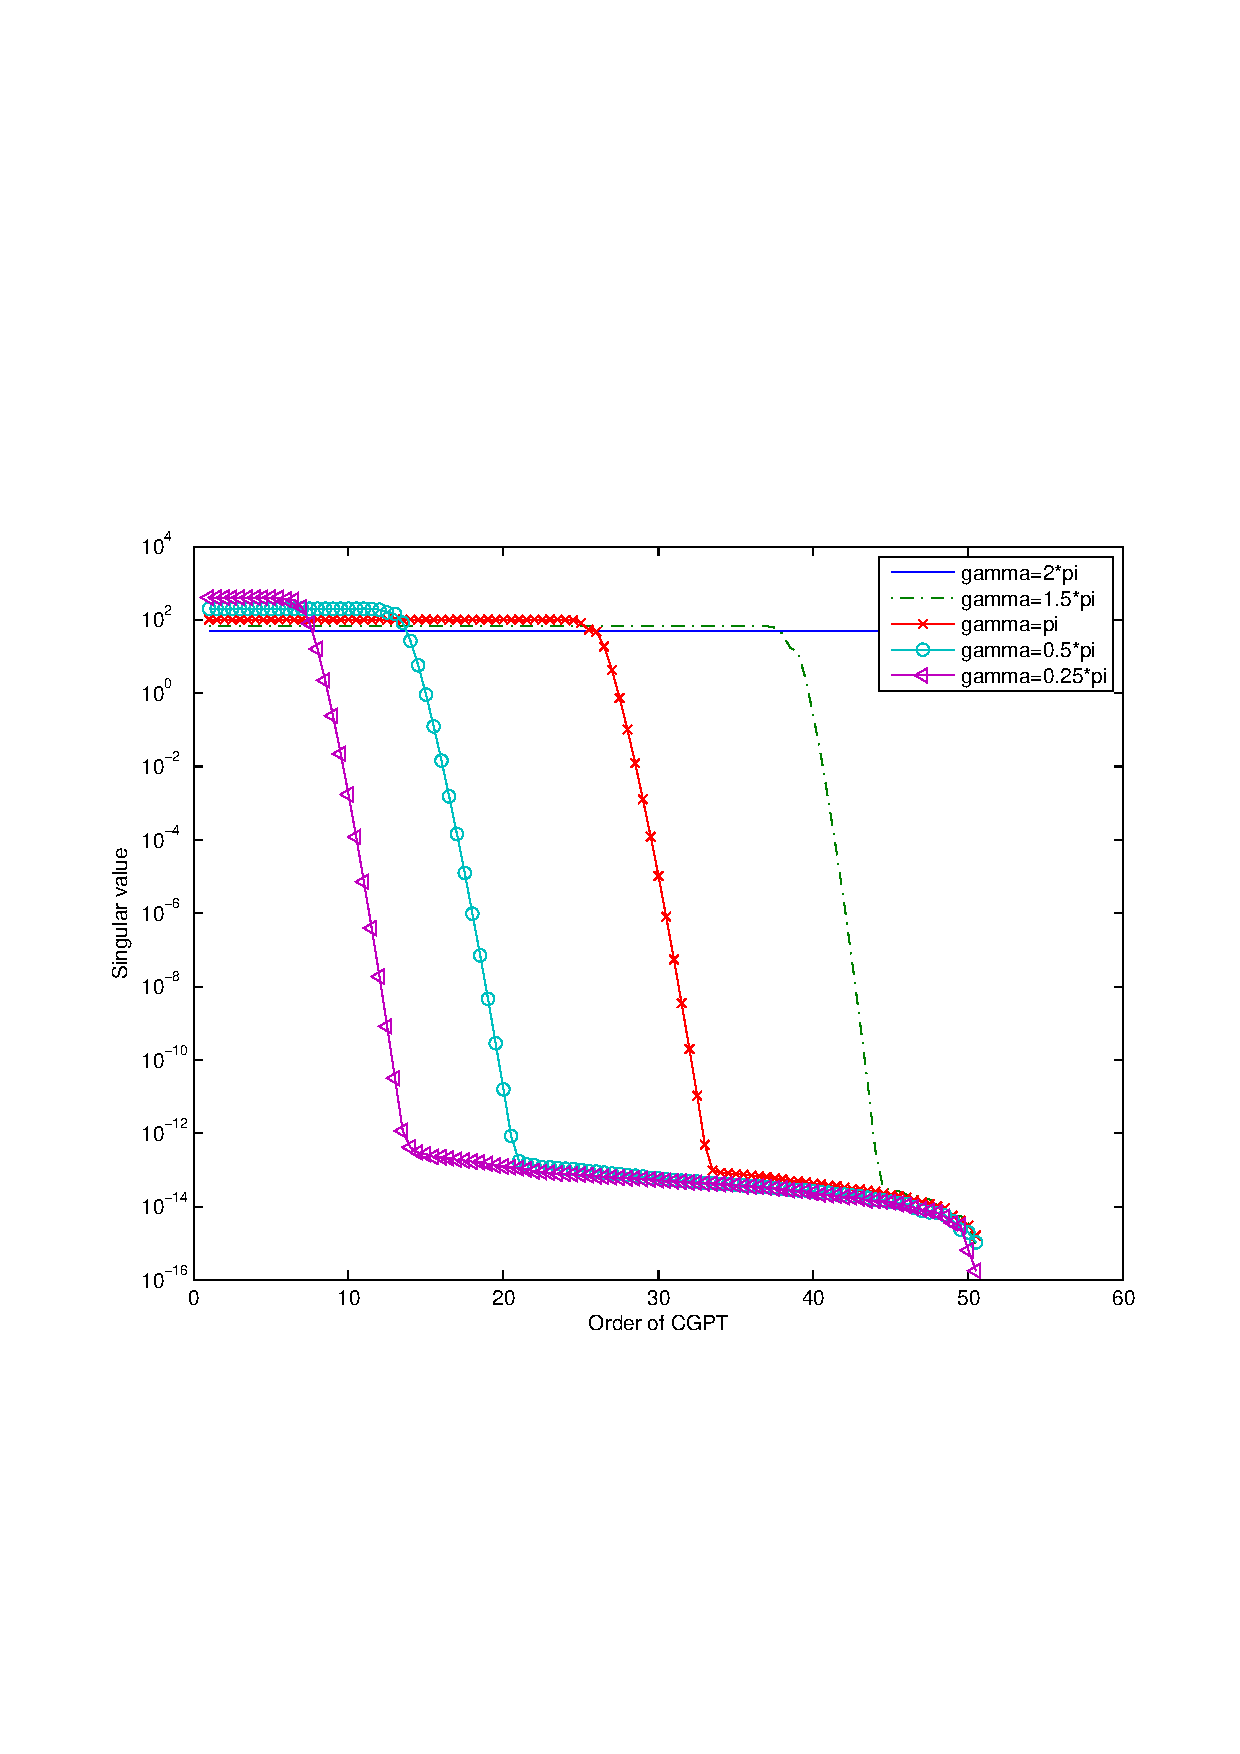
\includegraphics[width=0.45\textwidth]{tracking/cond_lim_aov/fig1a}}
  \subfigure[Eigenvalues of $\DCtCD$]{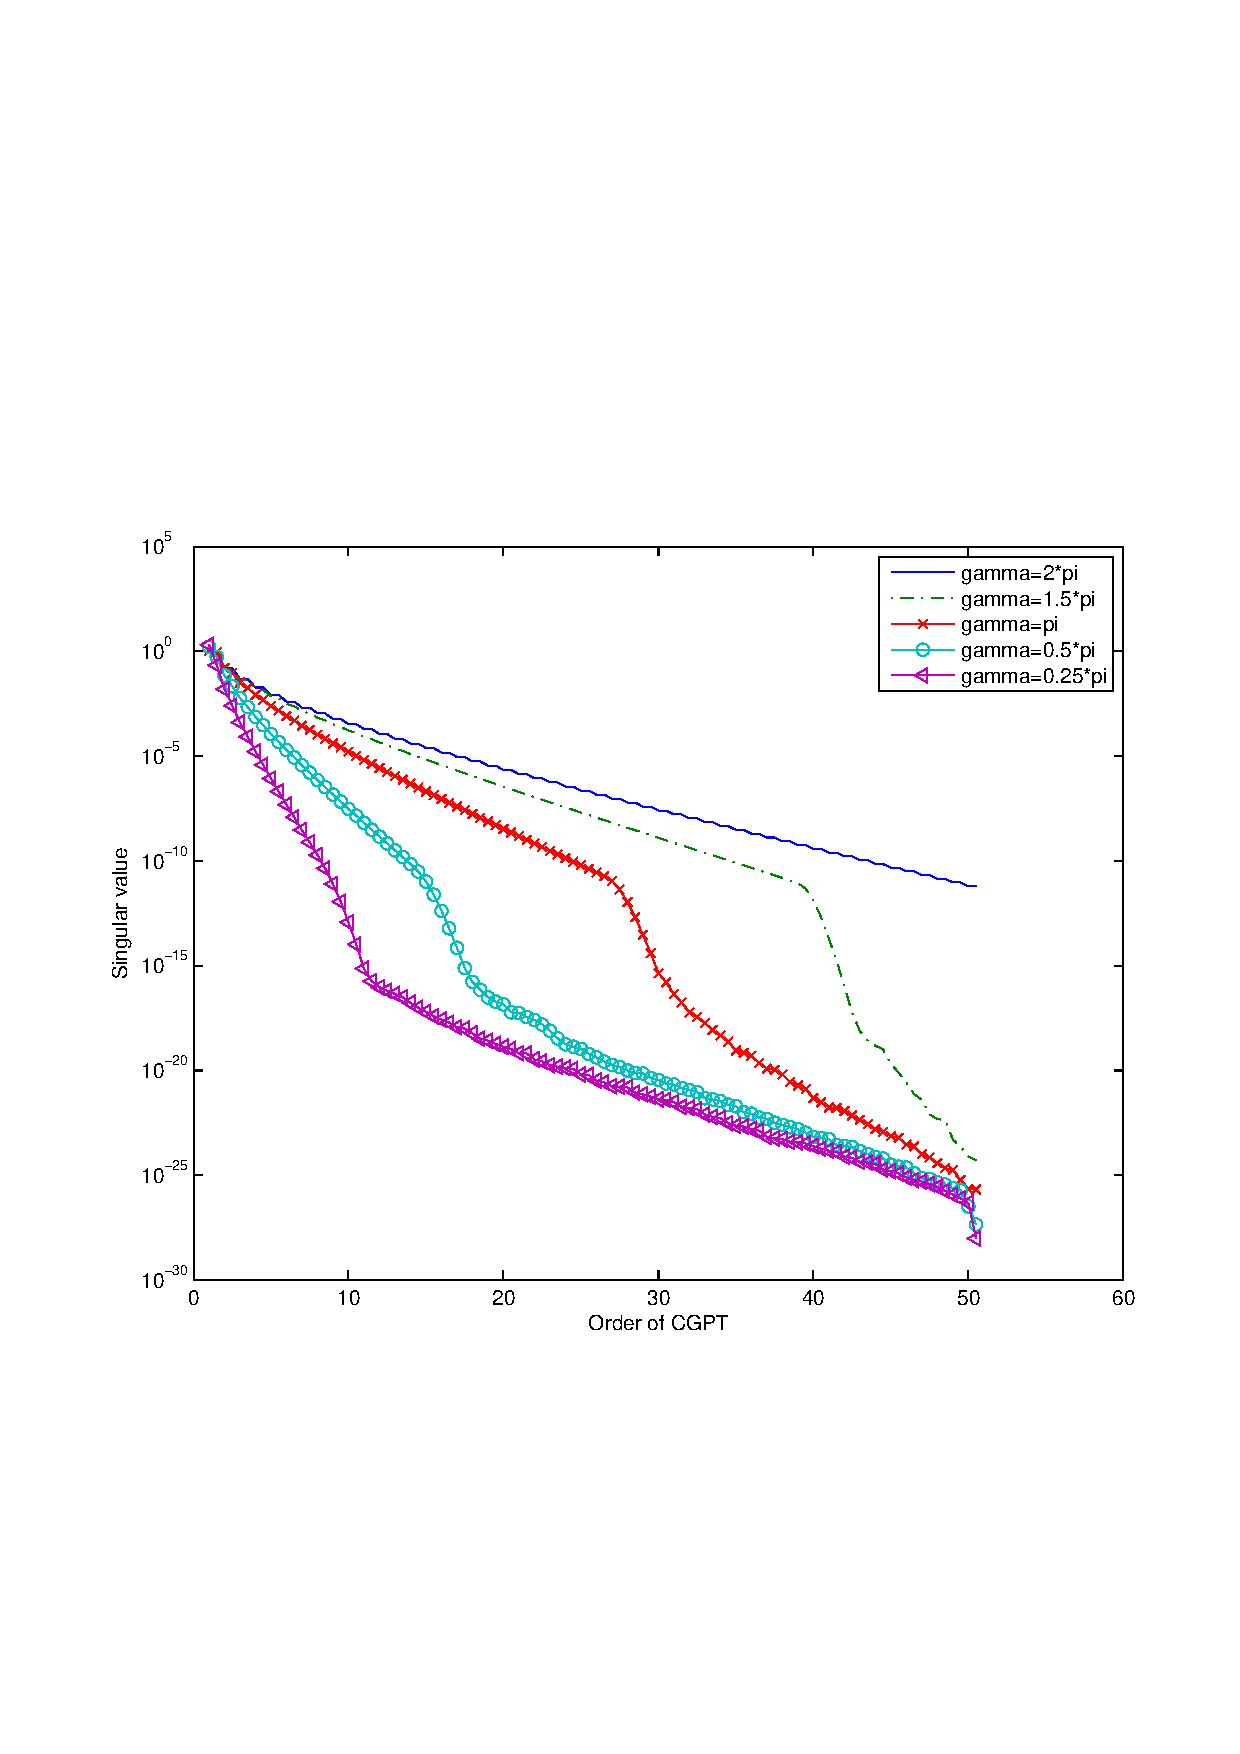
\includegraphics[width=0.45\textwidth]{tracking/cond_lim_aov/fig1b}}
  \caption{Distribution of eigenvalues (in log scale) of the matrix $\CtC$ (a) and $\DCtCD$
    (b). $N=101$ sources are equally spaced between $[0,\gamma)$ on a circle of radius $\rho=1.2$,
    and $K=50$. Each curve corresponds to a different value of $\gamma$. The matrix $\CtC$ and
    $\DCtCD$ are calculated from these parameters and their eigenvalues are sorted in decreasing
    order.}
  \label{fig:svd_CtC_DCtCD_gamma}
\end{figure}

\begin{figure}[htp]
  \centering
  \subfigure[Condition number of $\CtC$]{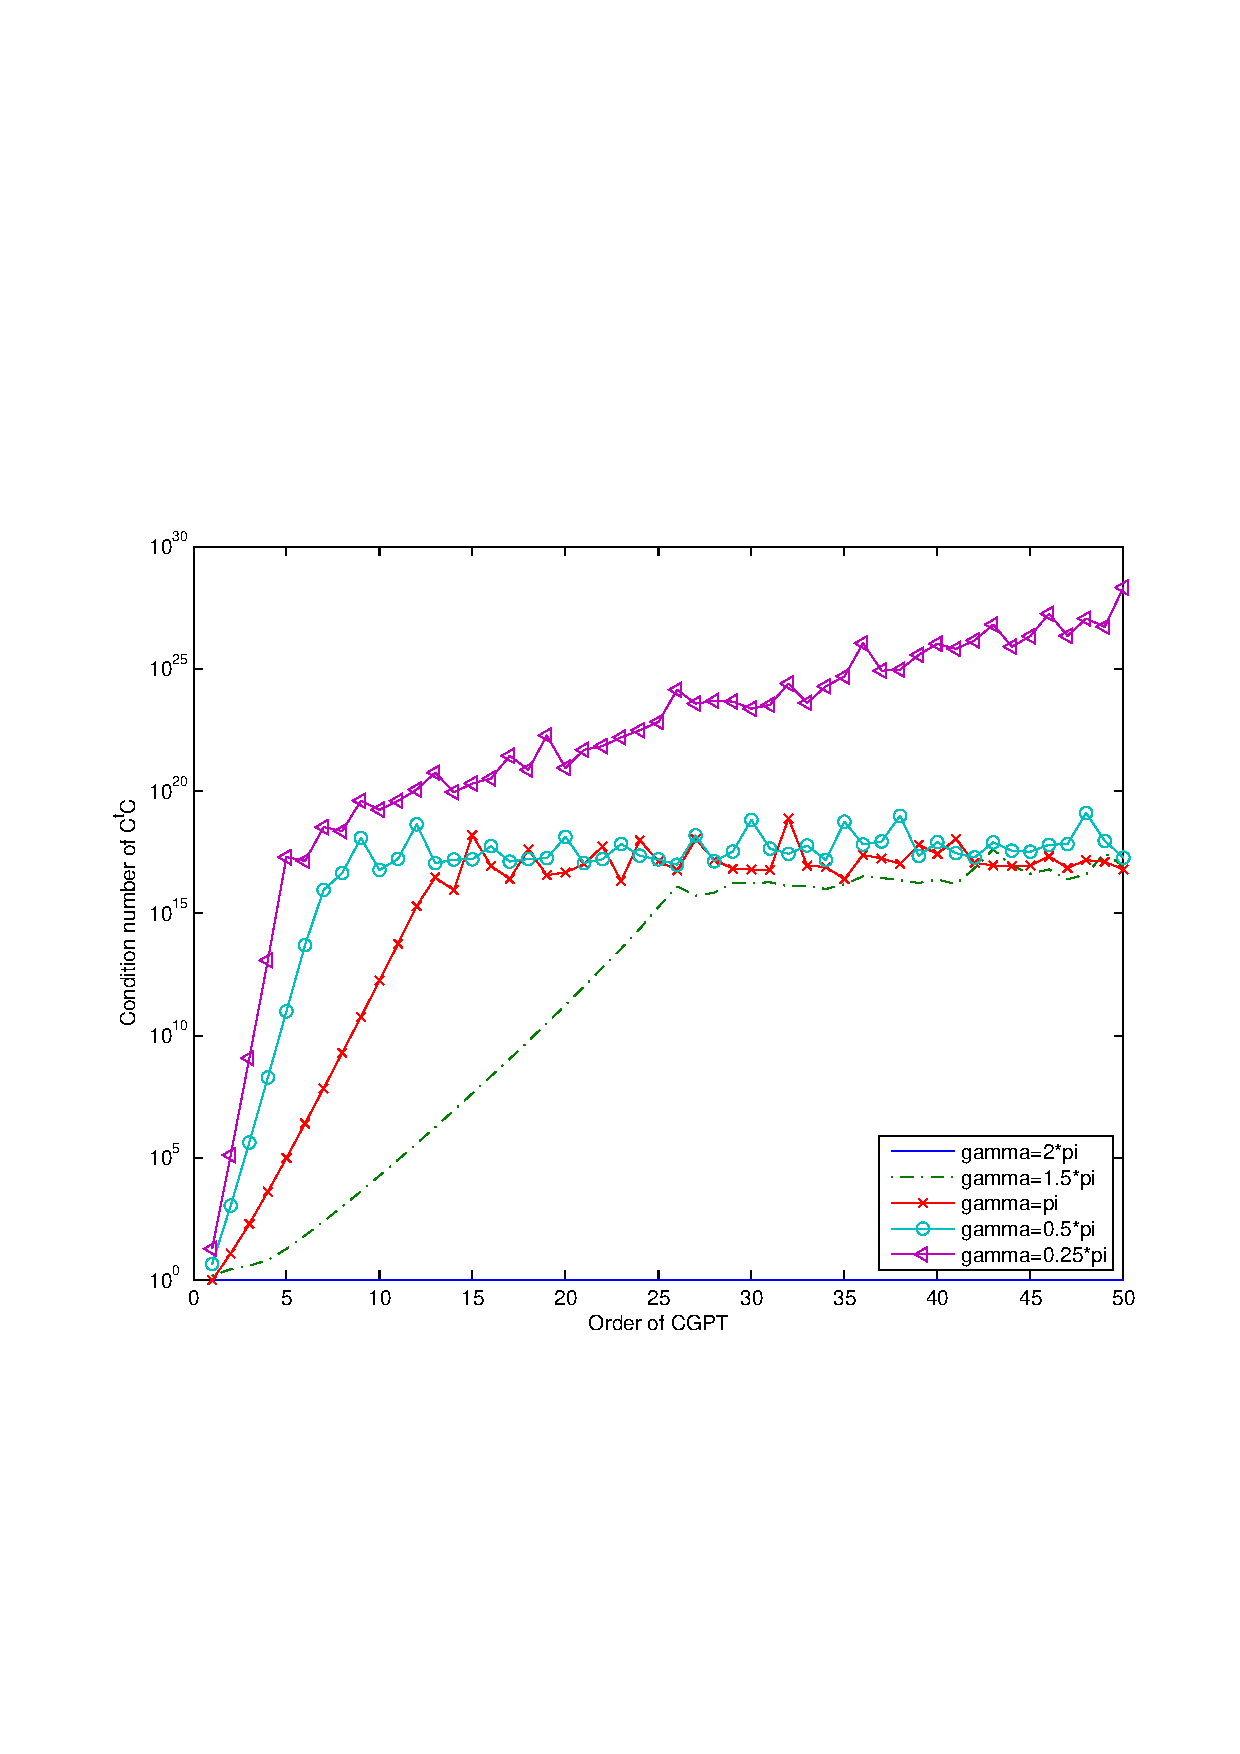
\includegraphics[width=0.45\textwidth]{tracking/cond_lim_aov/fig2a}}
  \subfigure[Condition number of $L$]{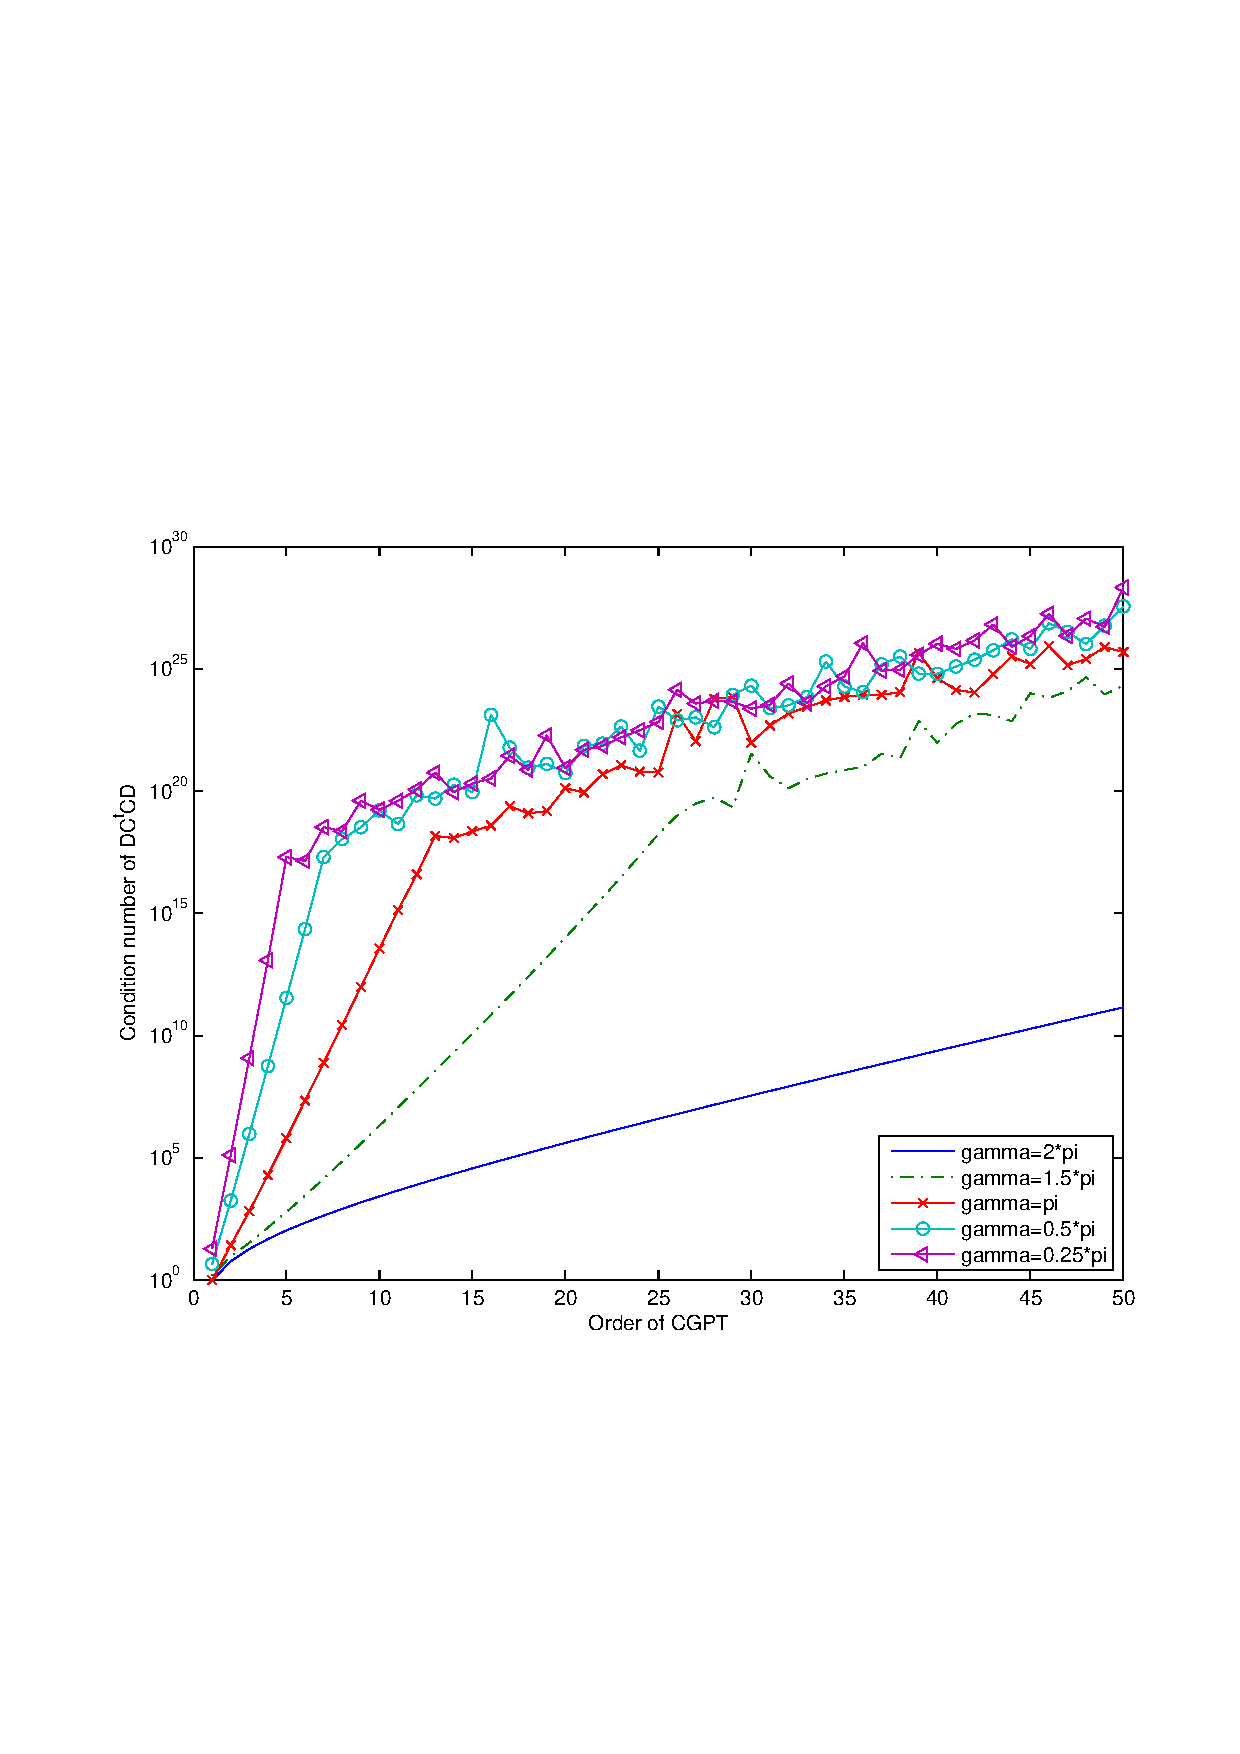
\includegraphics[width=0.45\textwidth]{tracking/cond_lim_aov/fig2b}}
  \subfigure[Condition number of $\CtC$]{\includegraphics[width=0.45\textwidth]{tracking/cond_lim_aov/fig3a}}
  \subfigure[Condition number of $L$]{\includegraphics[width=0.45\textwidth]{tracking/cond_lim_aov/fig3b}}
  \caption{Condition numbers (in log scale) of the matrix $\CtC$ (a) and the operator $L$ (b)
  for
    different orders $K$ between $[1,50]$. As in Figure~\ref{fig:svd_CtC_DCtCD_gamma}, $N=101$ sources
    are equally spaced between $[0,\gamma)$ on a circle of radius $\rho=1.2$. Figure(c) and (d) are
    the same experiment as Figure(a) and (b) but with $N=1001$.}
  \label{fig:svd_CtC_DCtCD_cond}
\end{figure}

% \begin{figure}[htp]
%   \centering
%   \subfigure[Condition number of $\CtC$]{\includegraphics[width=7.5cm]{fig3a}}
%   \subfigure[Condition number of $L$]{\includegraphics[width=7.5cm]{fig3b}}
%   \caption{Same experience as Figure~\ref{fig:svd_CtC_DCtCD_cond} but with $N=1001$, the other
%     parameters are the same.}
%   \label{fig:svd_CtC_DCtCD_cond_N501}
% \end{figure}

% We reconstruct the CGPT of an ellipse with a limited angle of view setting and compare the result
% with theoretical values.

% \begin{figure}[htp]
%   \centering
%   \subfigure[$N=101, \gamma=1.5\pi$]{\includegraphics[width=7.5cm]{../figures/101_1p5pi.eps}}
%   \subfigure[$N=101, \gamma=\pi$]{\includegraphics[width=7.5cm]{../figures/101_1pi_5_10_20_30.eps}}
%   \subfigure[$N=101, \gamma=0.5\pi$]{\includegraphics[width=7.5cm]{../figures/101_0p5pi_2_3_5_7_9.eps}}
%   \subfigure[$N=101, \gamma=0.25\pi$]{\includegraphics[width=7.5cm]{../figures/101_0p25pi_2_3_5_7_9.eps}}
%   \caption{Singular values of $\CtC$. In each figure, the curves from left to right correspond to the different value of $K$: Figure(a),
%     $K=10,20,30,40,50$, Figure(b): $K=5,10,20,30$, Figure(c) and (d): $K=2,3,5,7,9$.}
%   \label{fig:svd_CtC}
% \end{figure}

% Even for $\gamma$ close the eigen values
% There are several remarkable points in these results:
% \begin{itemize}
% \item The singular values always start by a constant part, then a sharp drop and finish by a tiny
%   tail. These tiny singular values disappear only when $K$ is small enough, which means that in
%   practice the matrix $\CtC$ is extremely ill-conditioned and numerically singular at the order of
%   $N/2$.
% \item For $\gamma$ fixed, as $K$ decreases, the singular value remains the same in the constant part while the tiny tail is removed.
% \item For small $\gamma$, the matrix is more ill-conditioned.
% \end{itemize}





\section{Numerical Results}

\label{sec:results-GPT-extraction}

In this section we present a variety of numerical results on the
theoretical framework discussed in this chapter with noisy MSR  measurements. Given a shape
$D_0$ of characteristic size $\delta$, the procedure of our
numerical experiment can be summarized as follows:
\begin{enumerate}
\item Data simulation. $N$ sources (and also receivers) are
equally
  distributed on a circle of radius $R$, which is centered at an
  arbitrary point $z_0\in D_0$ and includes $D_0$, see Figure
  \ref{fig:data_acq}. The MSR matrix is obtained by evaluating
  numerically its integral expression \eqref{eq:dfield} then adding a
  white noise of variance $\zeta^2$. For simplicity, here
  we suppose that the reference point $z_0\in D_0$ can be estimated by
  means of  algorithms such as MUSIC (standing for MUltiple SIgnal Classification) \cite{AGJ, ammari2007polarization}.
\item Reconstruction of the CGPTs of $D=D_0-z_0$ using formula
  \eqref{eq:Mest} or the least squares algorithm \eqref{eq:lsqr-GPT-reconstruction}.
\end{enumerate}
We emphasize that the reconstructed CGPTs of shape $D$ depend on
the reference point $z_0$. We fix the conductivity parameter
$k=4/3$ throughout this section.

\begin{figure}[htp]
  \centering
  \includegraphics[width=.4\textwidth]{dico/figures/fig1_ellipse_std}
  \caption{An example of the configuration for MSR data
    simulation. The unknown shape is an ellipse whose long and short
    axes are 2 and 1, respectively. $N=51$ sources/receivers (marked by
    ``x'') are equally placed on a circle of radius $R=2$ centered at
    $z_0=[0,0]$ (marked by ``*'').}
  \label{fig:data_acq}
  % [58.2, 37.9]
\end{figure}

\subsection{Reconstruction of CGPTs}\label{sec:reconstruction-cgpt}
The theoretical analysis presented in section
\ref{sec:reconstr-cgpt-stab} suggests the following two steps
method for the reconstruction of CGPTs. First we apply
\eqref{eq:Mest} (or equivalently solve the least squares
problem~\eqref{eq:lsqr-GPT-reconstruction}) by fixing the truncation order $K$ as in
\eqref{eq:nregime}:
\begin{align}
  % \frac{\log(\sigma/N)}{\log\rho}-2 < K < N/2
  K \leq \min\left ( \frac{\log(\zeta/N)}{\log\rho}-2, N/2\right
  ).
  \label{eq:max_trunc_ord}
\end{align}
% Here, $\zeta$ is the standard deviation of the
% measurement noise and $\rho = \delta/R$ with $\delta$ being the
% characteristic size of the target and $R$ the distance between the
% target center and the circular array of transmitters/receivers.
Then, we keep  only the first $m_0$ orders in the reconstructed
CGPTs, with $m_0$ being the resolving order deduced from
estimation \eqref{eq:snrest}:
\begin{align}
  m_0 =
  \frac{\log\zeta - \log \tau_0}{2\log\rho}, \label{eq:max_CGPT_order}
\end{align}
and $\tau_0\leq 1$ is the tolerance number introduced in
(\ref{eq:msdef}). In all our numerical experiments we set the
noise level $\zeta$ to:
\begin{align}
  \label{eq:noise_model}
  \zeta = (\V_{\mbox{max}} -
  \V_{\mbox{min}})\sigma_0,
\end{align}
with a positive constant $\sigma_0$ and $\V_{\mbox{max}}$ and
$\V_{\mbox{min}}$ being the maximal and the minimal coefficient in
the MSR matrix $\V$. Using the configuration given in
Figure~\ref{fig:data_acq} and for various noise level, we
reconstruct the CGPTs of the ellipse up to a truncation order $K$
which is determined as in \eqref{eq:max_trunc_ord}. For each $k
\leq K$, the relative error of the first $k$-th order
reconstructed CGPTs is evaluated by comparing with their
theoretical value (\cite[Proposition
4.7]{ammari2007polarization}). The results are shown in
Figure~\ref{fig:err_rec_CGPT}. In Figure
\ref{fig:rslv_ord_rel_err_CGPT} we plot the resolving order $m_0$
given by \eqref{eq:max_CGPT_order} and the relative error of the
reconstruction within this order, for $\sigma_0$ in the range
$[10^{-3}, 1]$.

% \begin{remark}
%   \textcolor{red}{We remark that,
%   due to the special form of \eqref{eq:Mest}, the CGPTs reconstructed
%   in this way are the same as those by taking $K=m_0$ in
%   \eqref{eq:Mest} directly.}
% \end{remark}

% \begin{align}
%   \label{eq:CGPT_recon_rel_err}
%   \mbox{error}_{\mbox{rel}} := \frac{\Mcgpt_{k}-\Mcgpt^0_{k}}{\norm{}}
% \end{align}
% of the reconstructed CGPT is obtained
\begin{figure}[htp]
  \centering
  \subfigure[$\sigma_0=0.01, m_0=6$]{\includegraphics[width=.45\textwidth]{dico/figures/fig2_0p01.eps}}
  \subfigure[$\sigma_0=0.1, m_0=4$]{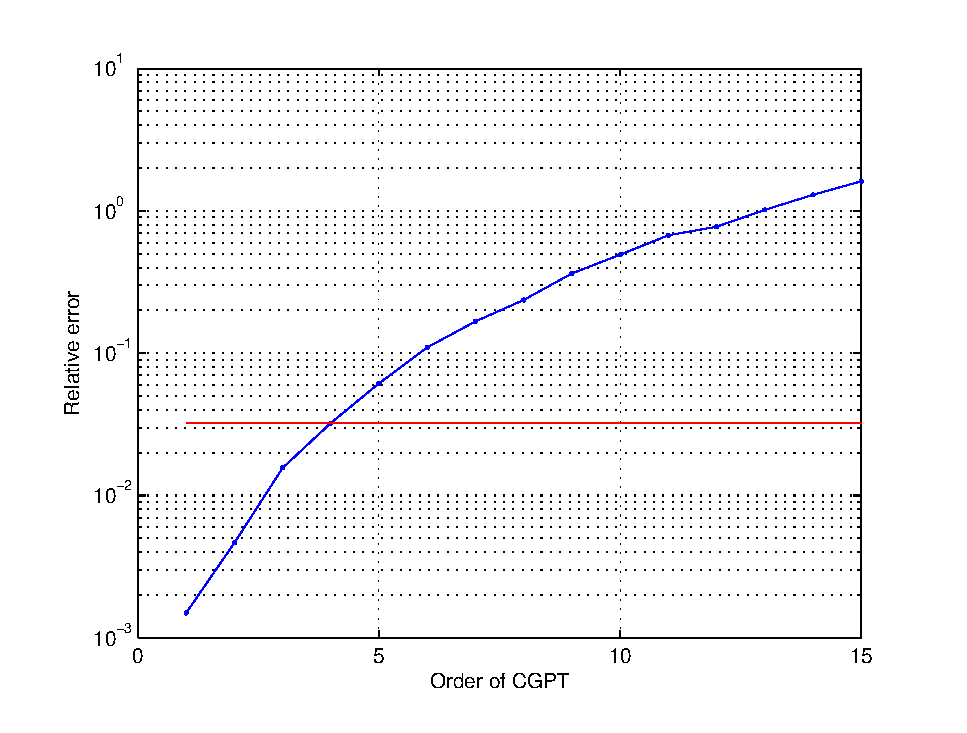
\includegraphics[width=.45\textwidth]{dico/figures/fig2_0p1.eps}}
  \subfigure[$\sigma_0=0.5, m_0=3$]{\includegraphics[width=.45\textwidth]{dico/figures/fig2_0p5.eps}}
  \subfigure[$\sigma_0=1.0, m_0=2$]{\includegraphics[width=.45\textwidth]{dico/figures/fig2_1p0.eps}}
  \caption{Relative error of the reconstructed CGPTs. For each noise
    level, we repeat the experiment 100 times (corresponding to 100 realizations of the noise) and the
    reconstruction is taken as their mean value. The horizontal solid
    line in each figure indicates the resolving order $m_0$ given by
    \eqref{eq:max_CGPT_order} with the tolerance number $\tau_0=10^{-1}$.}
  \label{fig:err_rec_CGPT}
\end{figure}

\begin{figure}[htp]
  \centering
  \subfigure[Resolving order]{\includegraphics[width=.45\textwidth]{dico/figures/fig3_b.eps}}
  \subfigure[Relative error]{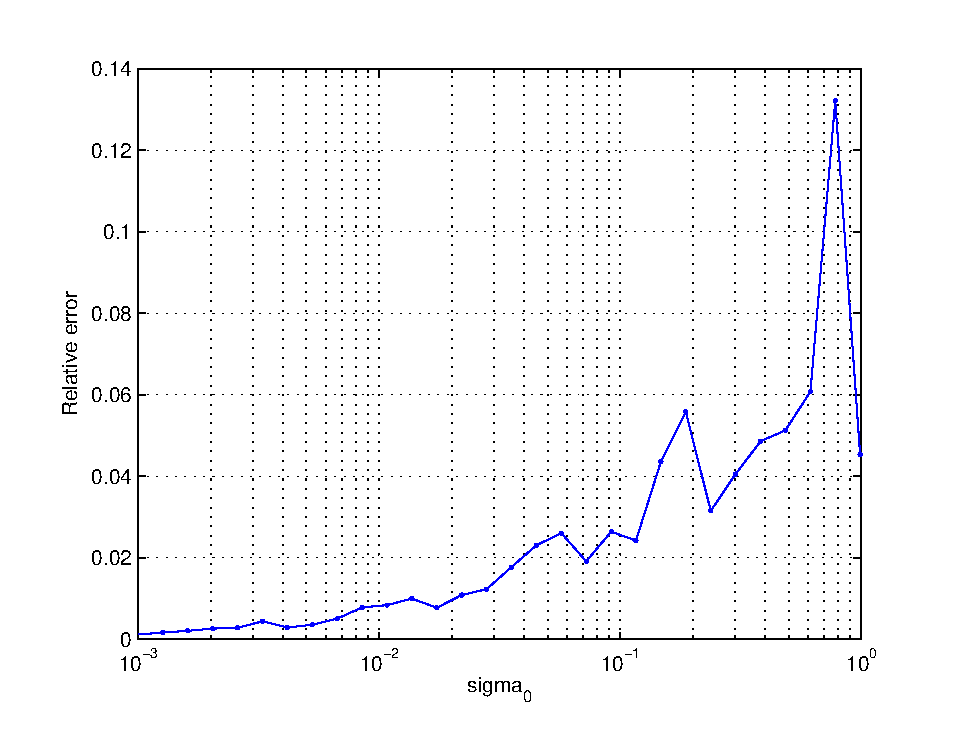
\includegraphics[width=.45\textwidth]{dico/figures/fig3_a.eps}}
  \caption{The resolving order $m_0$, for $\sigma_0\in[10^{-3},1], \tau_0=10^{-1},$ and
    the relative error of the reconstruction within this order. As in
    Figure~\ref{fig:err_rec_CGPT}, we repeat the experiment 100
    times and the reconstruction is taken as their mean value. The
    large variations of the relative error in (b) for $\sigma_0>10^{-1}$ indicate the
    instability of the reconstruction for very noisy data.}
  \label{fig:rslv_ord_rel_err_CGPT}
\end{figure}

\subsection{Partial View Setting}
\label{sec:recon_cgpt_num2}

The analysis performed in subsection~\ref{sec:limited_angle_view} suggests that the least-squares problem
\eqref{eq:lsqr-GPT-reconstruction} is not adapted to the CGPT
reconstruction in a limited-view setting. Actually, the truncation
error or the noise of measurement will be amplified by the tiny
singular values of $L$, and yields extremely instable
reconstruction of high-order CGPTs, {\it e.g.}, $K\geq 2$.
Instead, we use
Thikhonov regularization and propose to solve
\begin{align}
  \label{eq:Least_square_reg_CGPT_recon}
    \min_{\bM}\  \norm{L(\bM) - \bV}_F^2 + \mu \norm{\bM}_F^2,
\end{align}
with $\mu>0$ a small regularization constant. It is well known
that the effect of the regularization term is to truncate those
singular values of $L$ smaller than $\mu$, which consequently
stabilizes the solution. The optimal choice of $\mu$ depends on
the noise level, and here we determine it from the range
$[10^{-6}, 10^{-1}]$ by comparing the solution of
\eqref{eq:Least_square_reg_CGPT_recon} with the true CGPTs.

Here we reconstruct the CGPTs of an ellipse with the parameter
$N=101, K=50$, and $\gamma$ varying between 0 and $2\pi$.  The
major and minor axis of the ellipse are 1 and 0.5 respectively. In
Figure~\ref{fig:cgpt_lim_aov} we show the error of the first 2 order
CGPTs reconstructed through \eqref{eq:Least_square_reg_CGPT_recon}
and \eqref{eq:lsqr-GPT-reconstruction} at three different noise
levels. It can be seen that, for small $\gamma$, the error
obtained by \eqref{eq:Least_square_reg_CGPT_recon} is
substantially smaller.

%\graphicspath{{../figures/CGPT_lim_aov/}}
\begin{figure}[htp]
  \centering
  \subfigure[]{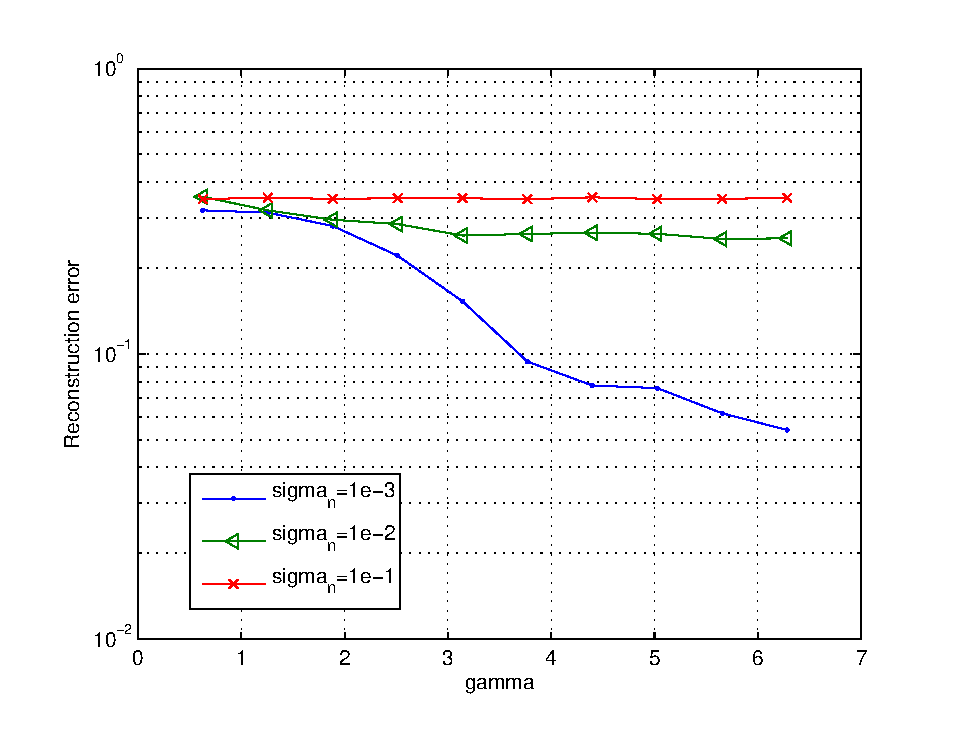
\includegraphics[width=.45\textwidth]{tracking/CGPT_lim_aov/fig1a}}
  \subfigure[]{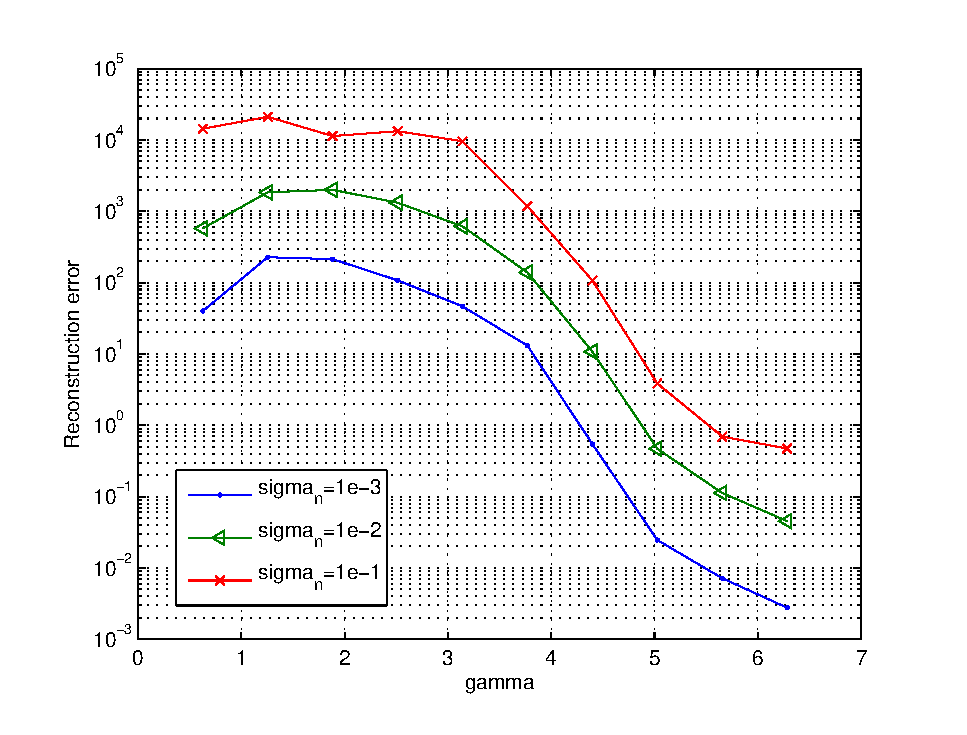
\includegraphics[width=.45\textwidth]{tracking/CGPT_lim_aov/fig1b}}
  \caption{Error of reconstructed CGPT of an ellipse compared with true CGPT values at different
    noise levels. We solve \eqref{eq:Least_square_reg_CGPT_recon} and
    \eqref{eq:lsqr-GPT-reconstruction} with $N=101, K=50$, and compare the first two orders with the
    true CGPT. The $x$-axis is the angle of view $\gamma$. Figure(a): results of
    \eqref{eq:Least_square_reg_CGPT_recon}, Figure(b): results of \eqref{eq:lsqr-GPT-reconstruction}.}
  \label{fig:cgpt_lim_aov}
\end{figure}

\section{Conclusion}

In this chapter, we have proposed a general framework for extraction of GPTs from
multi-static measurements.
From a least-squares formulation, we are able to extract those tensors from
multi-static measurements. We have analyzed the stbility of our algorithms with
respect to measurement noise, in the cases of full-view and partial-view setting.